\documentclass[12pt,letterpaper]{article}

\usepackage[utf8]{inputenc}
\usepackage{ragged2e}
\usepackage{amsfonts}
\usepackage{amssymb}
\usepackage{graphicx}
\usepackage{multicol}
\usepackage{changepage}
\usepackage{float}
\usepackage{cite}
\usepackage{url}
\usepackage[left=2.50cm, right=2.50cm]{geometry}
\usepackage[spanish]{babel}
\graphicspath{ {images/} }


\author{Ram\'irez Fuentes Edgar Alejandro}
\title{Entrega 2}
\date {2020-11-03}

\begin{document}
	%encabezado 
	\pagestyle{plain}
	{

		% Imágenes de la portada
		{
			\begin{tabular}
				{
					p{0.75\textwidth} 
					p{0.25\textwidth} 
				}
				
\includegraphics[width=1.5cm, height=2.5cm]{ipn.png} &  
				
\includegraphics[width=2.5cm, height=2cm]{escom.png}
			\end{tabular}
		}

		% Datos de la caratula
		\begin{center}

			\par\vspace{1cm} %Espacio dejado antes del encabezado
			{
				\Huge\textbf
				{
					Instituto Polit\'ecnico Nacional 
					\\[.2cm]Escuela Superior de C\'omputo
				}
			}

			\par\vspace{0.5cm}
			{
				\large\textbf
				{
					Ingenier\'ia en sistemas computacionales 
					\\[.5cm]An\'alisis y diseño orientado a objetos
				}
			}

			\vfill

			\par\vspace{0.7cm}
			{
				\textbf
				{
					Entrega 4 \\
                    CEDAE (Centro dermatológico de alta especialidad) \\
                    Mockups
				}
			}

			\vfill

			\par\vspace{0.7cm}
			{
				\textbf
				{
                    Equipo 3:
                    \\Angeles Hernández Jesús Eduardo
                    \\Chanes Nuñez Ricardo Jehonadab
                    \\García Gamiño Rafael Julian
                    \\Hernández Ceciliano Luis Ángel
                    \\Mendoza Cuellar José Oscar
                    \\Olvera Olvera Kevin Jesús
                    \\Paniagua Juárez Nadia Patricia
                    \\Ramírez Fuentes Edgar Alejandro
                    \\Zamorano Cruz Juan Raymundo
					\\2CV9
				} 
			}

			\par\vspace{3cm}

		\end{center}
		\clearpage
	}

	\newpage
	\tableofcontents
    \newpage

    \newpage
    
    \section{Objetivo}
    El proposito de este documento es mostrar al lector los prototipos de las interfaces para el sistema web de CEDAE.

    \section{Mockups}

        \subsection{Mockups generales}
        Página principal
            \begin{figure}[H]
                \centering
                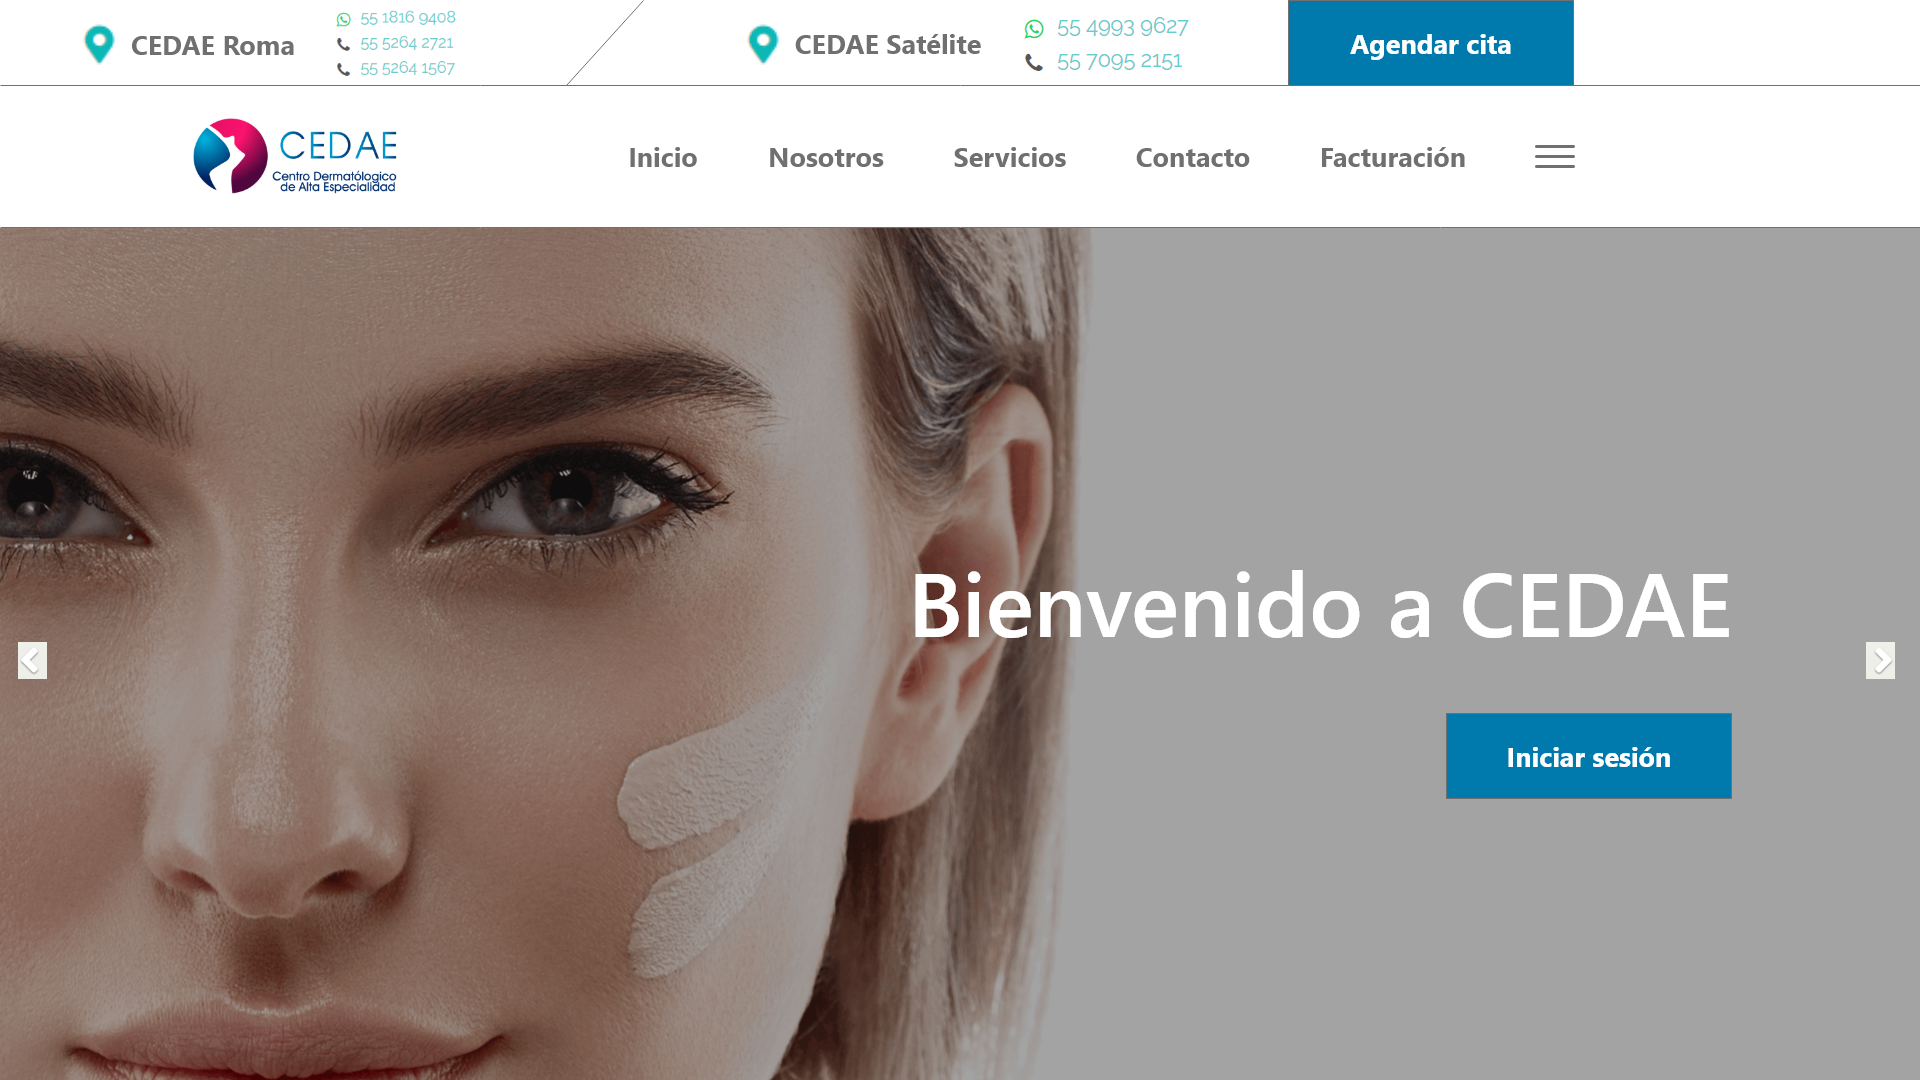
\includegraphics [scale=0.13]{gen_index}
                \caption{Interfaz de página principal}
            \end{figure}
        Iniciar sesión
            \begin{figure}[H]
                \centering
                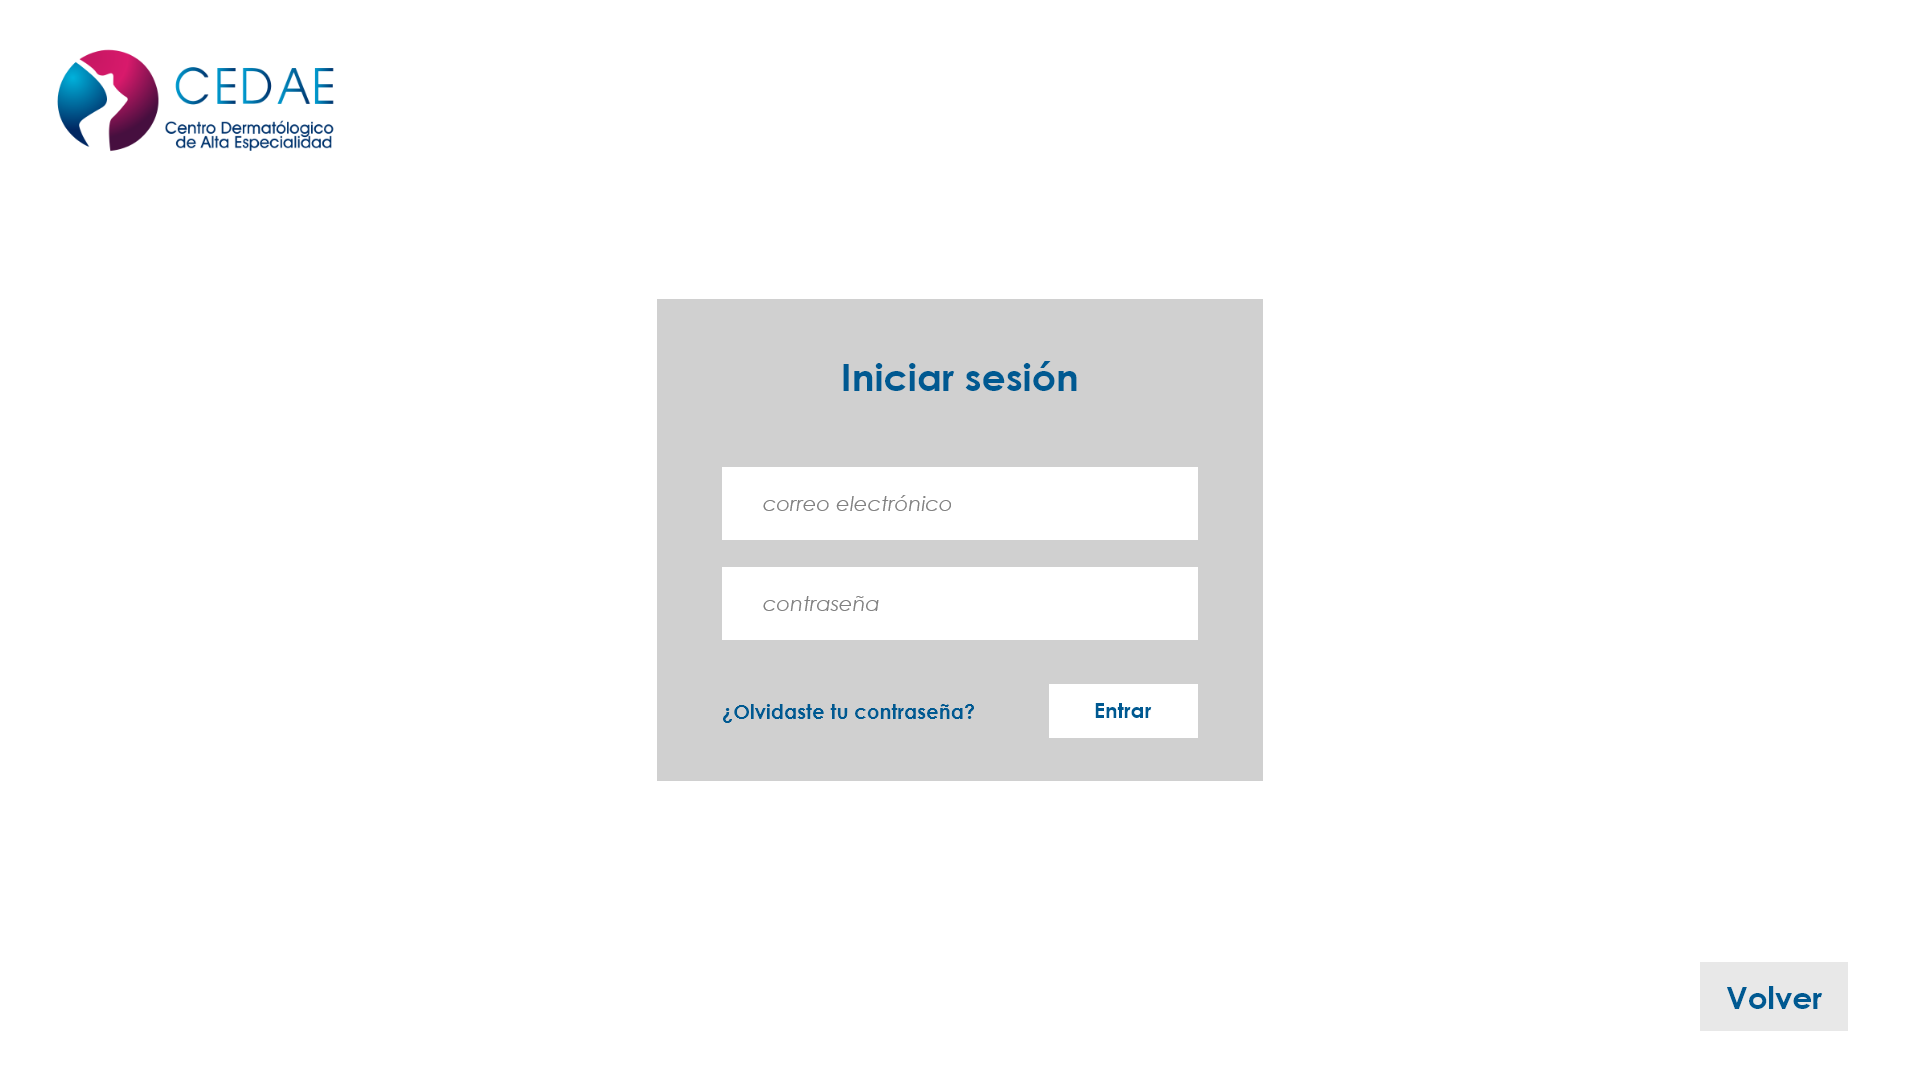
\includegraphics [scale=0.13]{gen_login}
                \caption{Interfaz de inicio de sesión}
            \end{figure}
        Recuperar contraseña
            \begin{figure}[H]
                \centering
                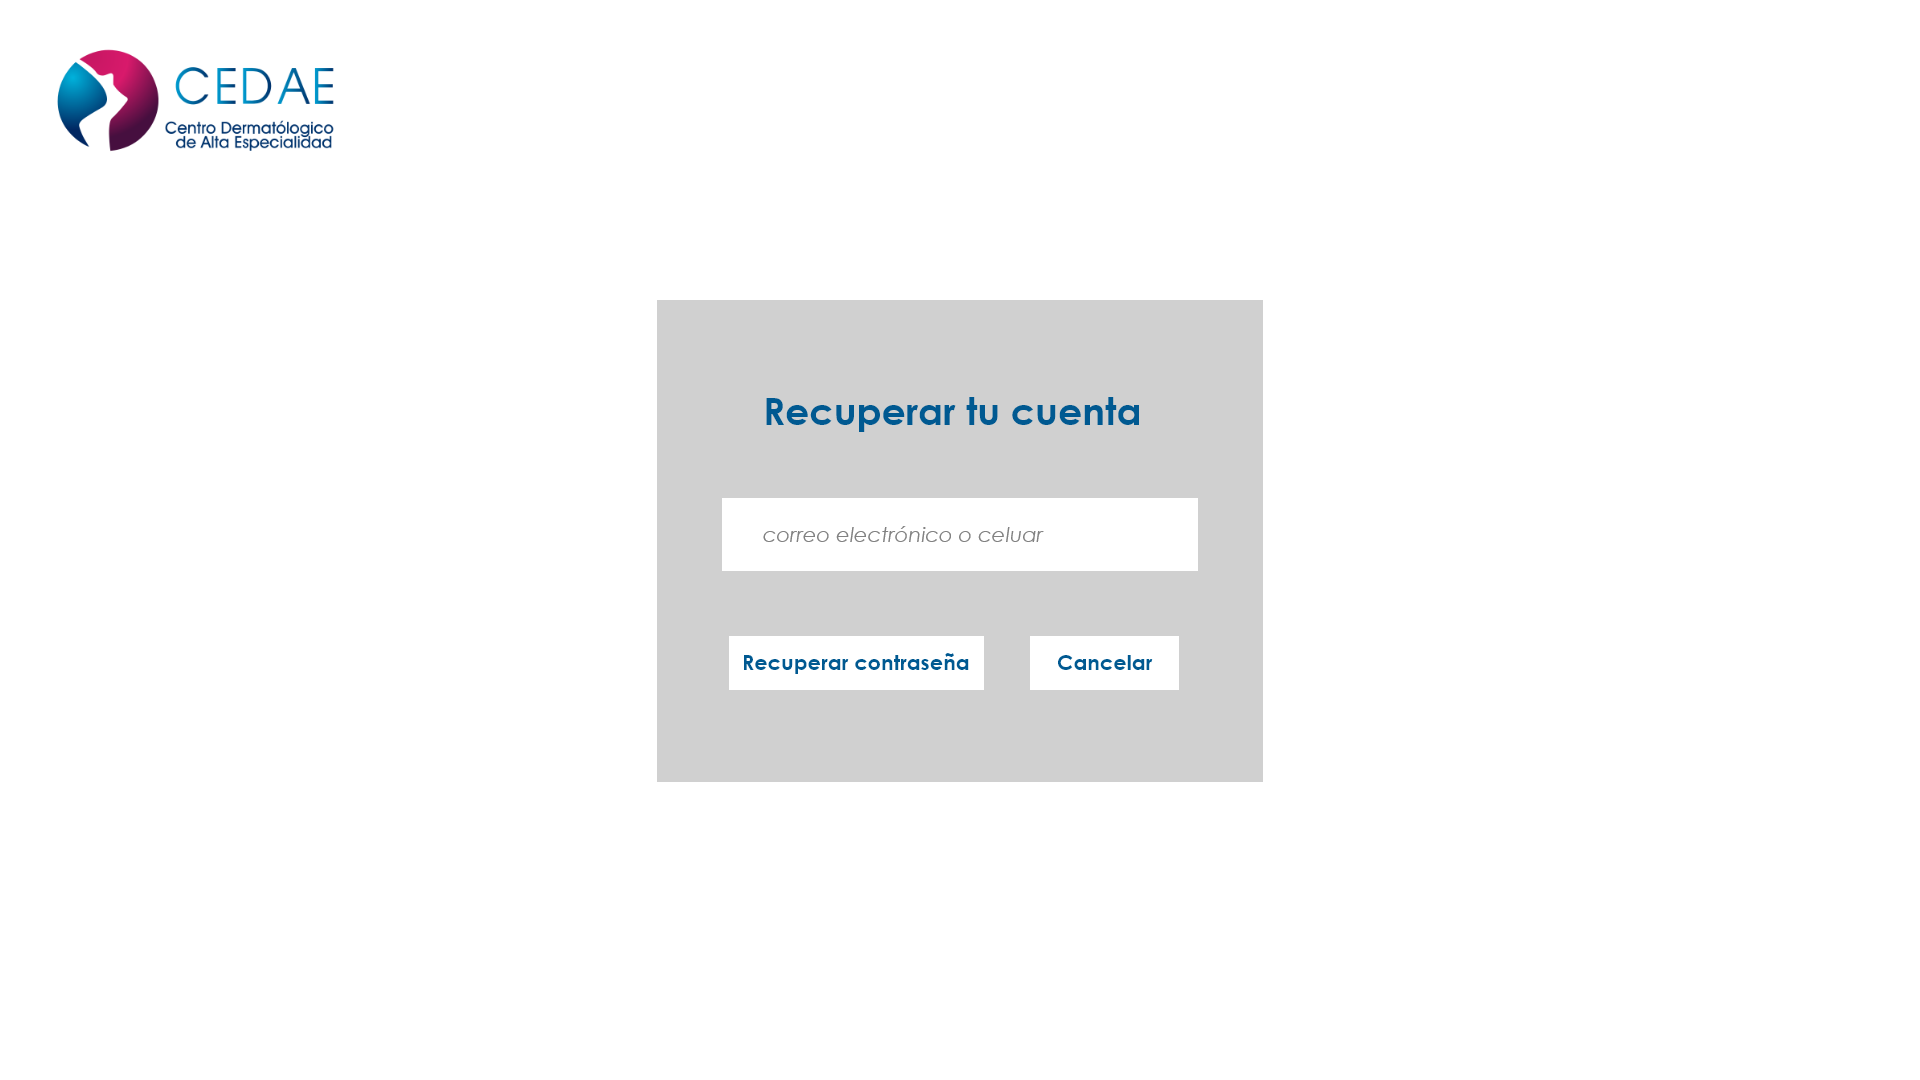
\includegraphics [scale=0.16]{gen_recovery}
                \caption{Interfaz de recuperación de contraseña}
            \end{figure}

        \subsection{Mockups de administrador}
        Perfil de administrador
            \begin{figure}[H]
                \centering
                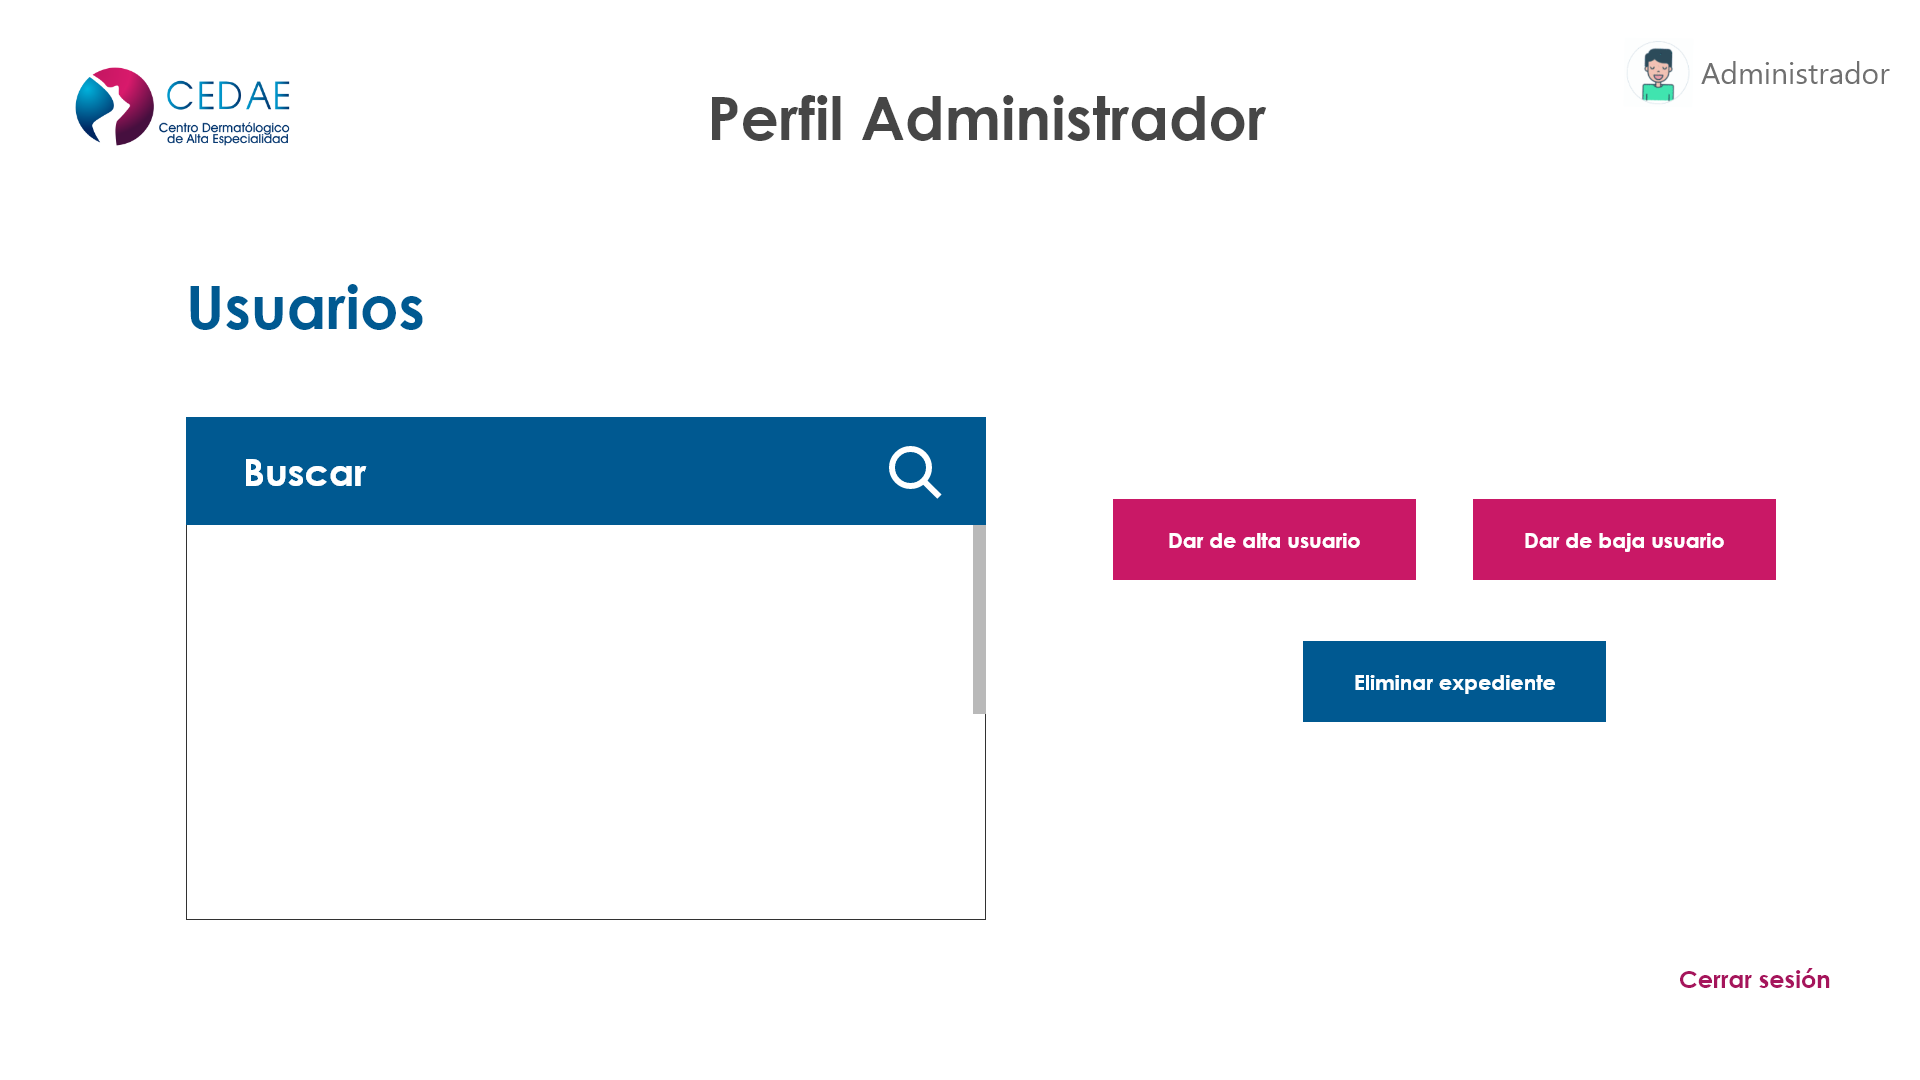
\includegraphics [scale=0.2]{adm_perfil}
                \caption{Interfaz de perfil de administrador}
            \end{figure}
        Registrar usuario
            \begin{figure}[H]
                \centering
                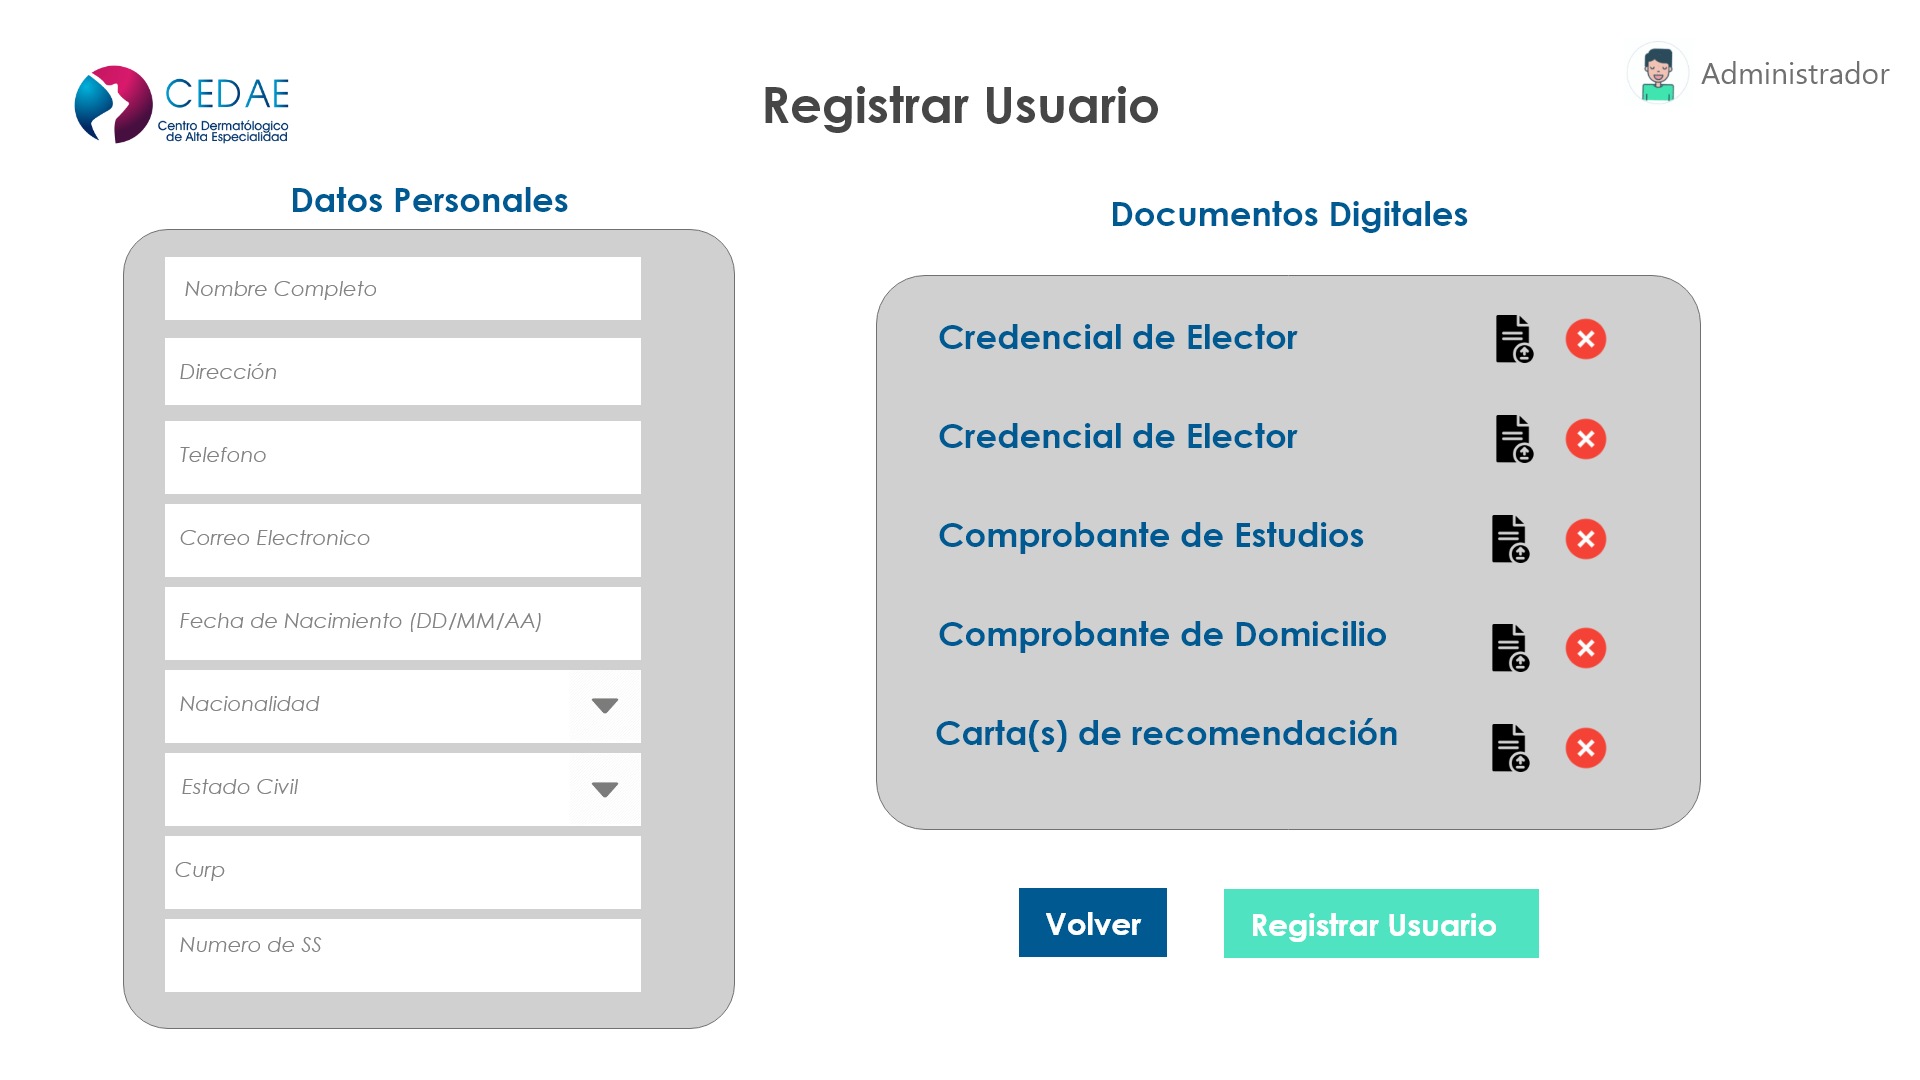
\includegraphics [scale=0.2]{adm_reg_usuario}
                \caption{Interfaz de registro de usuario}
            \end{figure}
        Dar de baja usuario
            \begin{figure}[H]
                \centering
                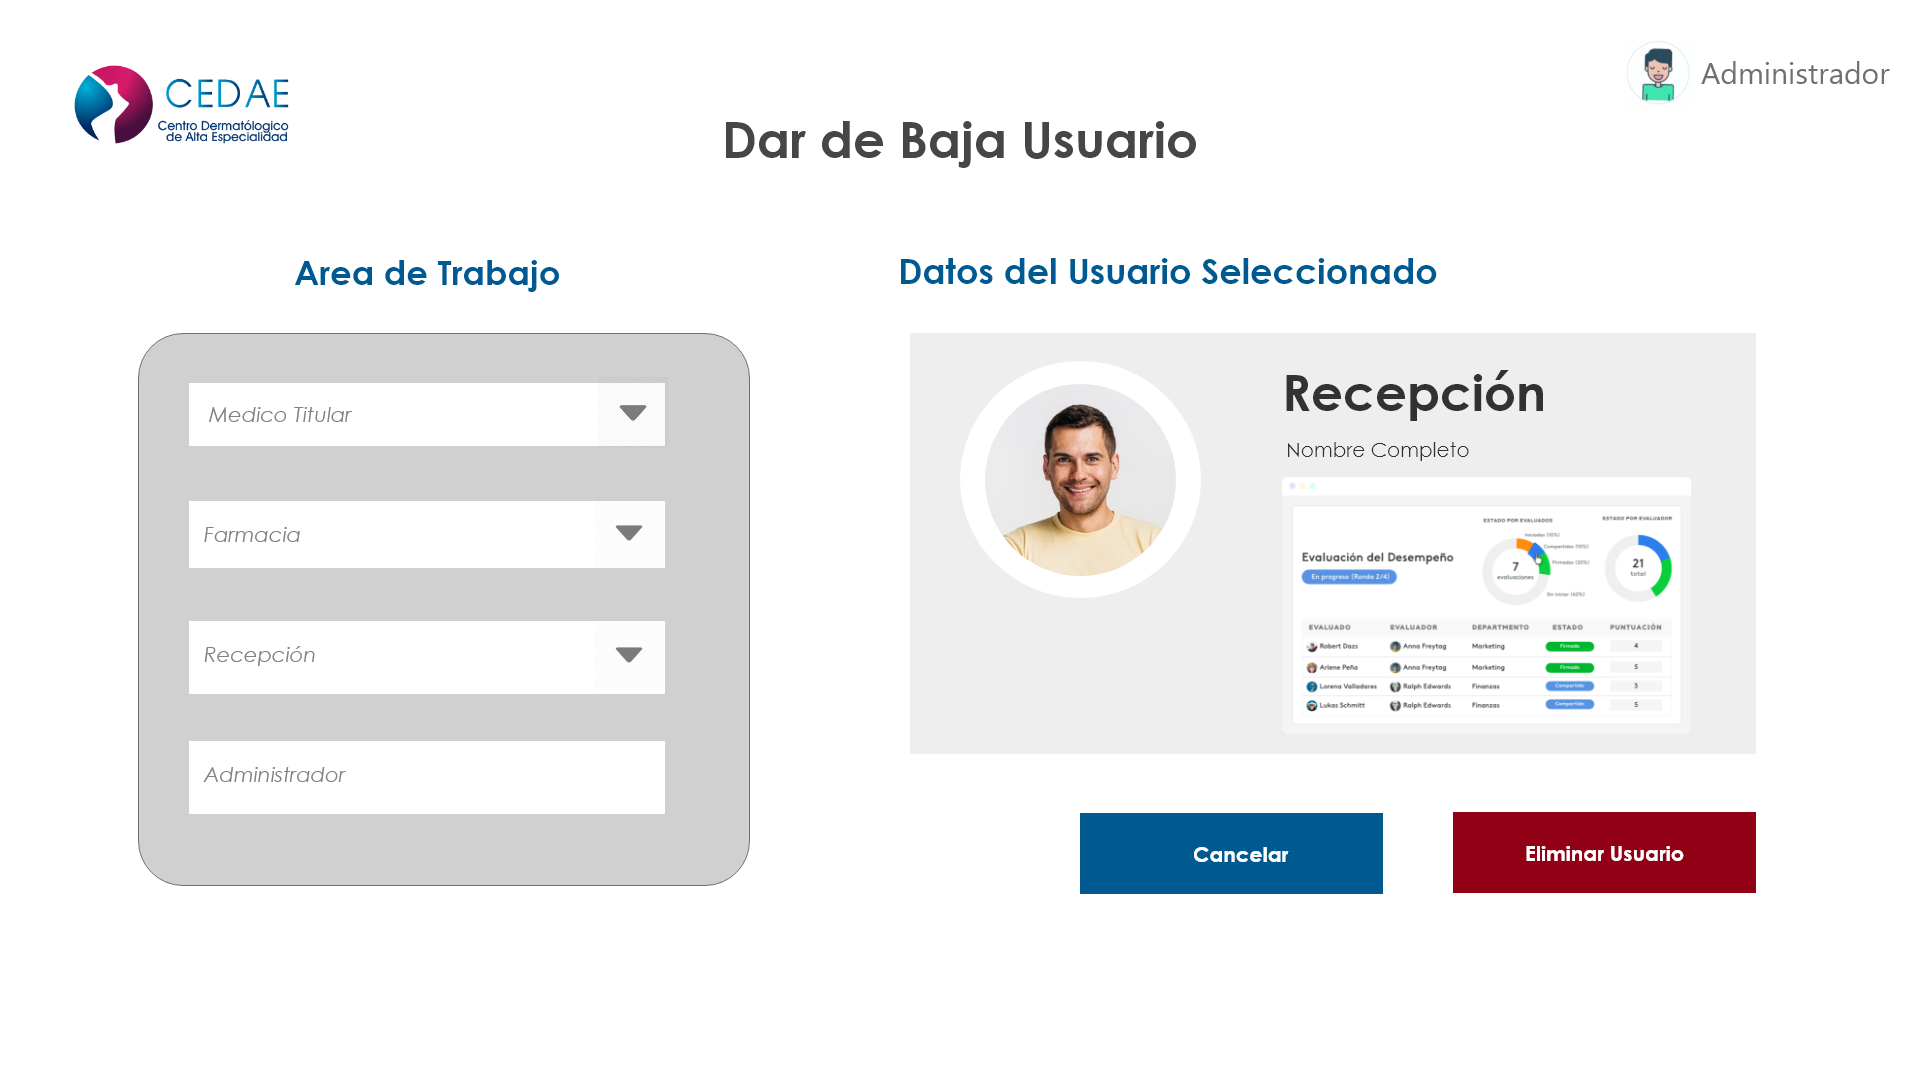
\includegraphics [scale=0.2]{adm_baja_usuario}
                \caption{Interfaz de baja de usuario}
            \end{figure}
        Modificar información de usuarios
            \begin{figure}[H]
                \centering
                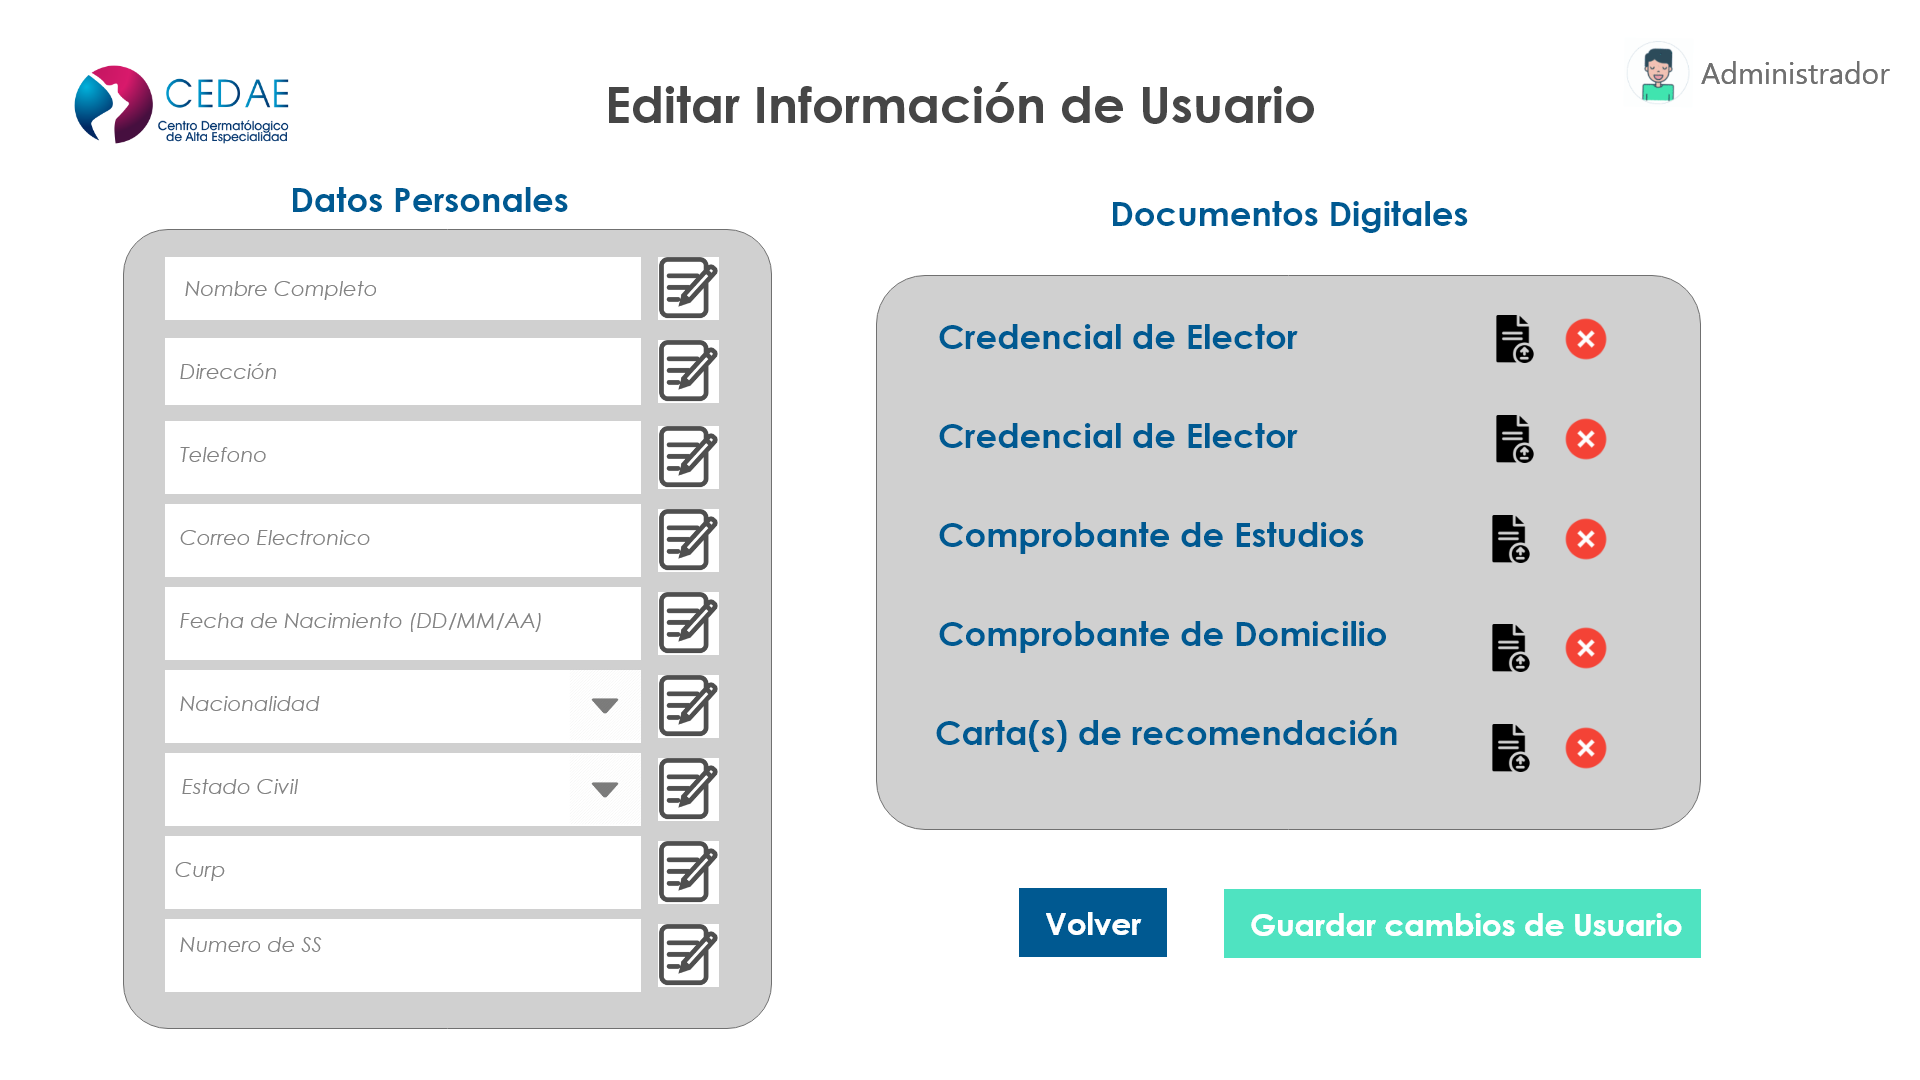
\includegraphics [scale=0.2]{adm_mod_info}
                \caption{Interfaz de modificación de información de usuario}
            \end{figure}
        Ver usuarios registrados
            \begin{figure}[H]
                \centering
                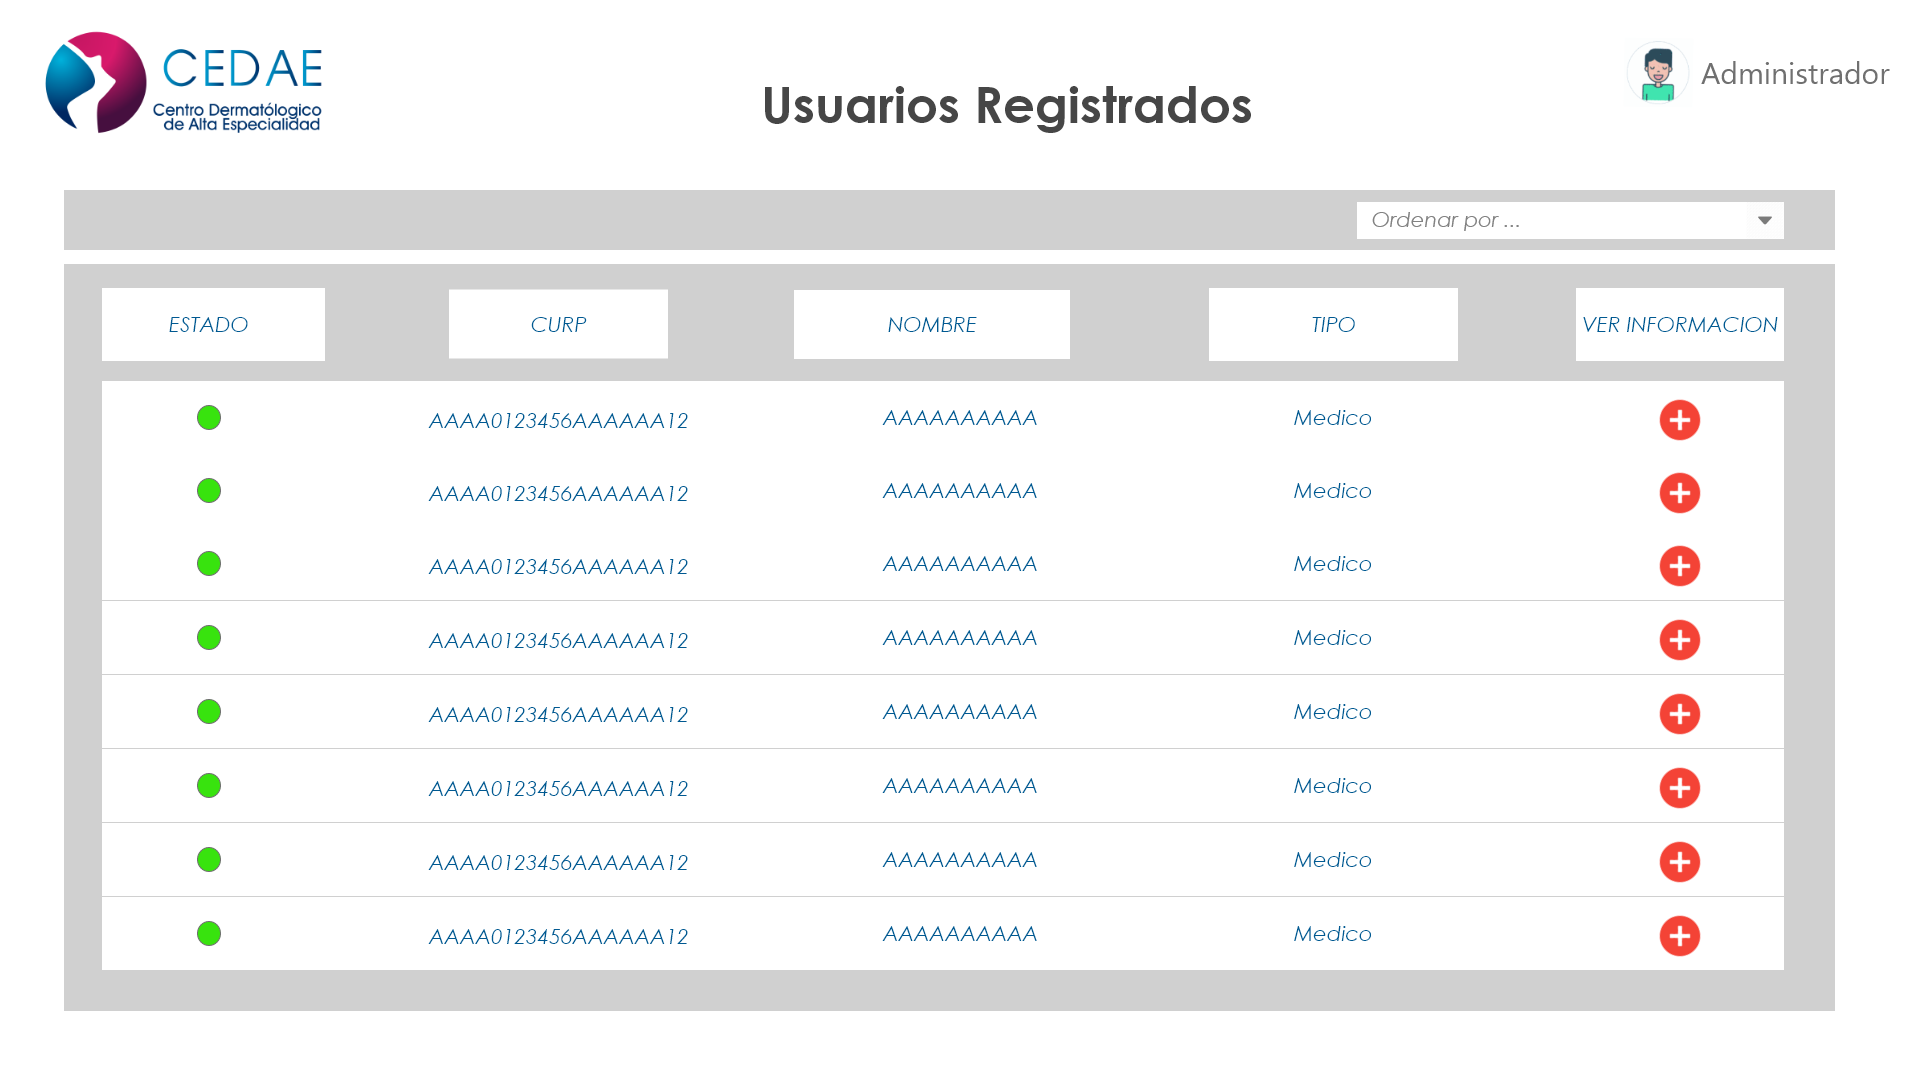
\includegraphics [scale=0.2]{adm_ver_usuario}
                \caption{Interfaz de usuarios registrados}
            \end{figure}

        \subsection{Mockups de encargado de farmacia}
        Perfil de encargado de farmacia
            \begin{figure}[H]
                \centering
                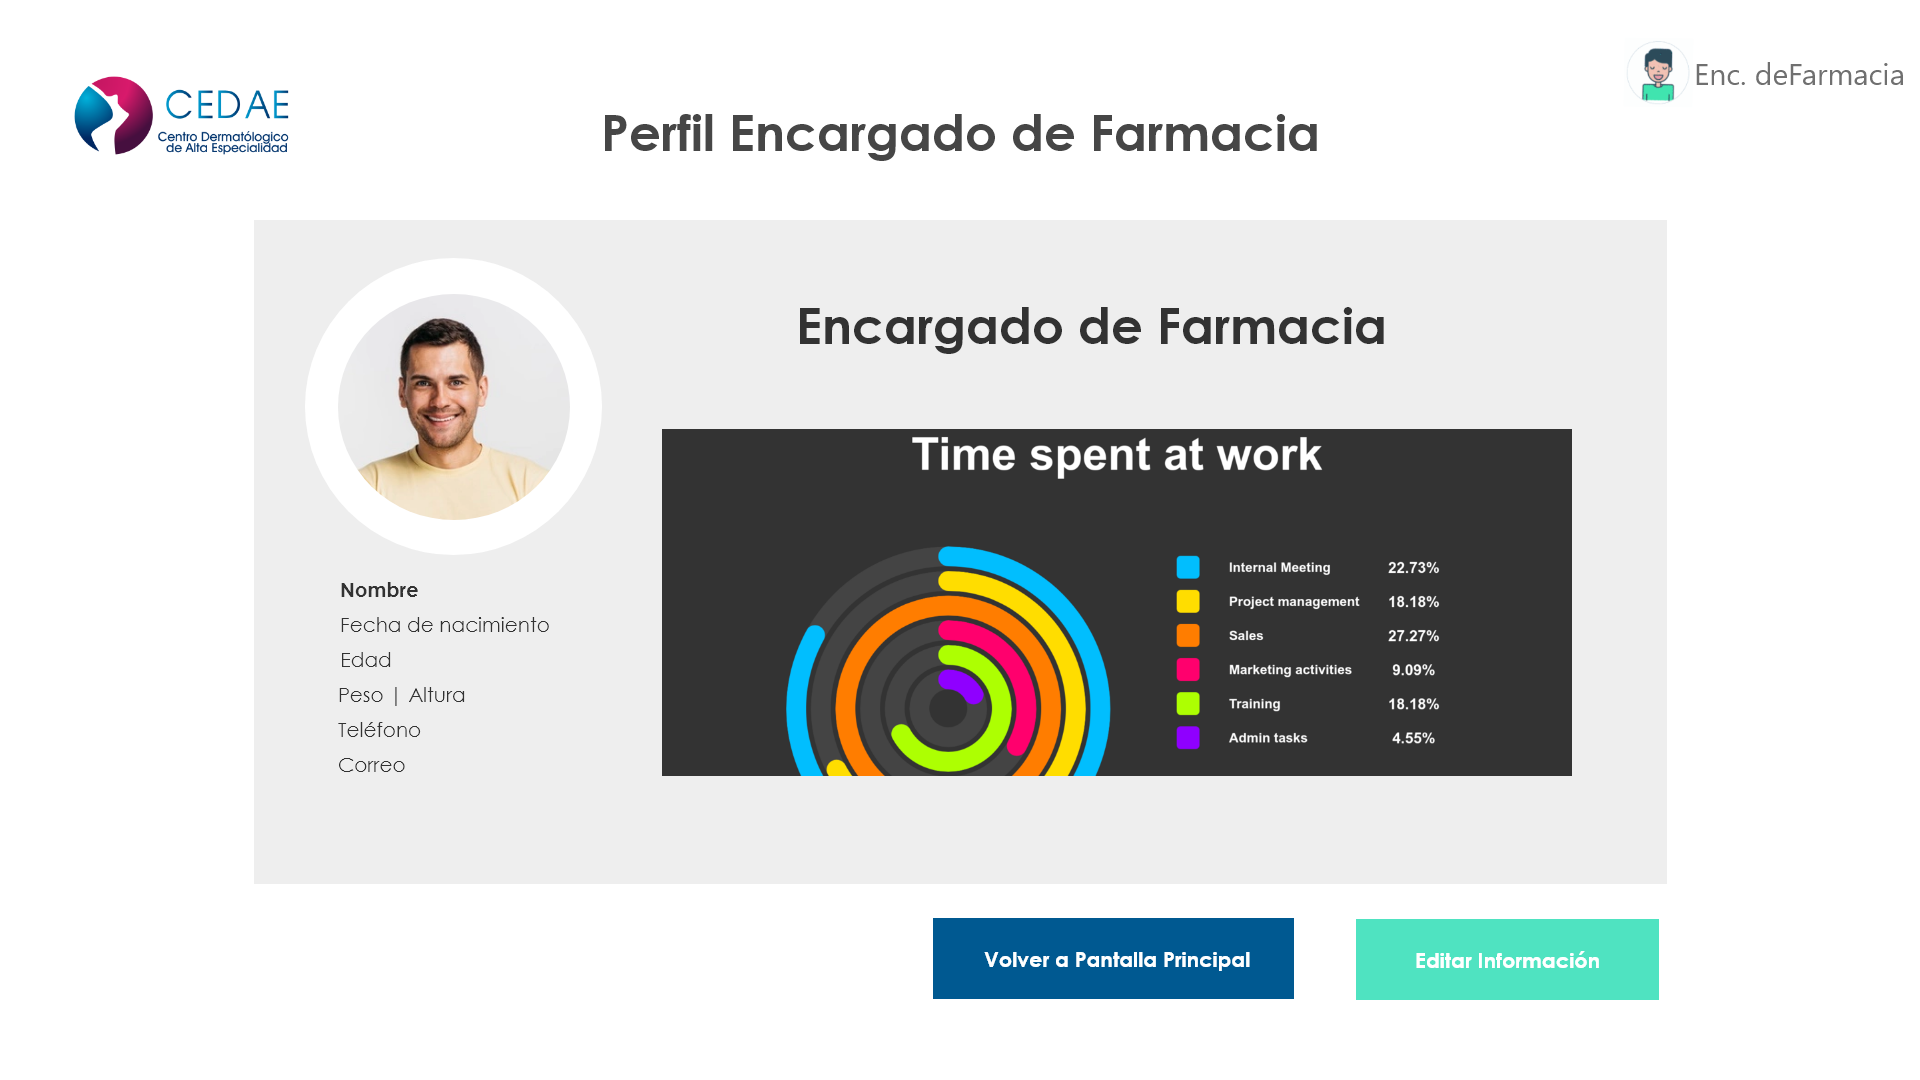
\includegraphics [scale=0.19]{far_perfil}
                \caption{Interfaz de perfil de encargado de farmacia}
            \end{figure}
        Inventario de medicamentos
            \begin{figure}[H]
                \centering
                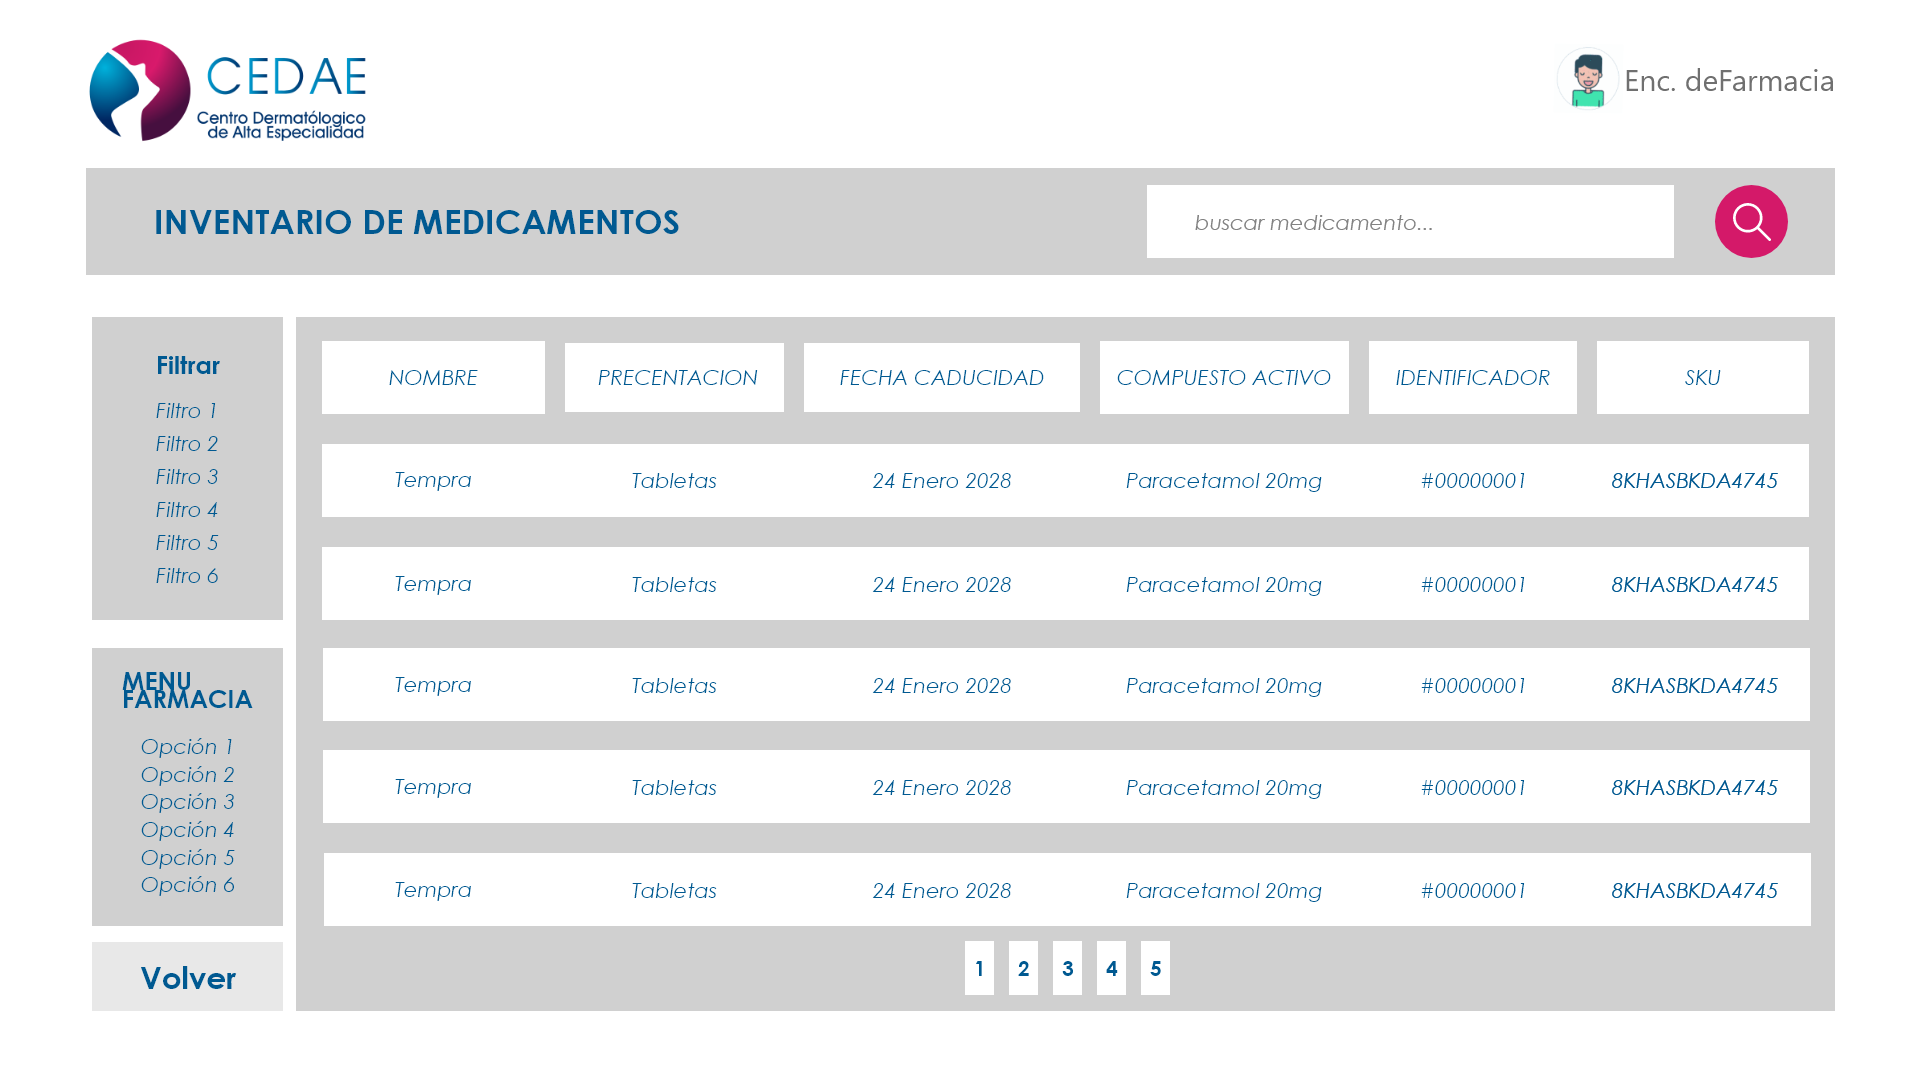
\includegraphics [scale=0.18]{far_inv_medicamento}
                \caption{Interfaz de inventario}
            \end{figure}
        Agregar medicamentos
            \begin{figure}[H]
                \centering
                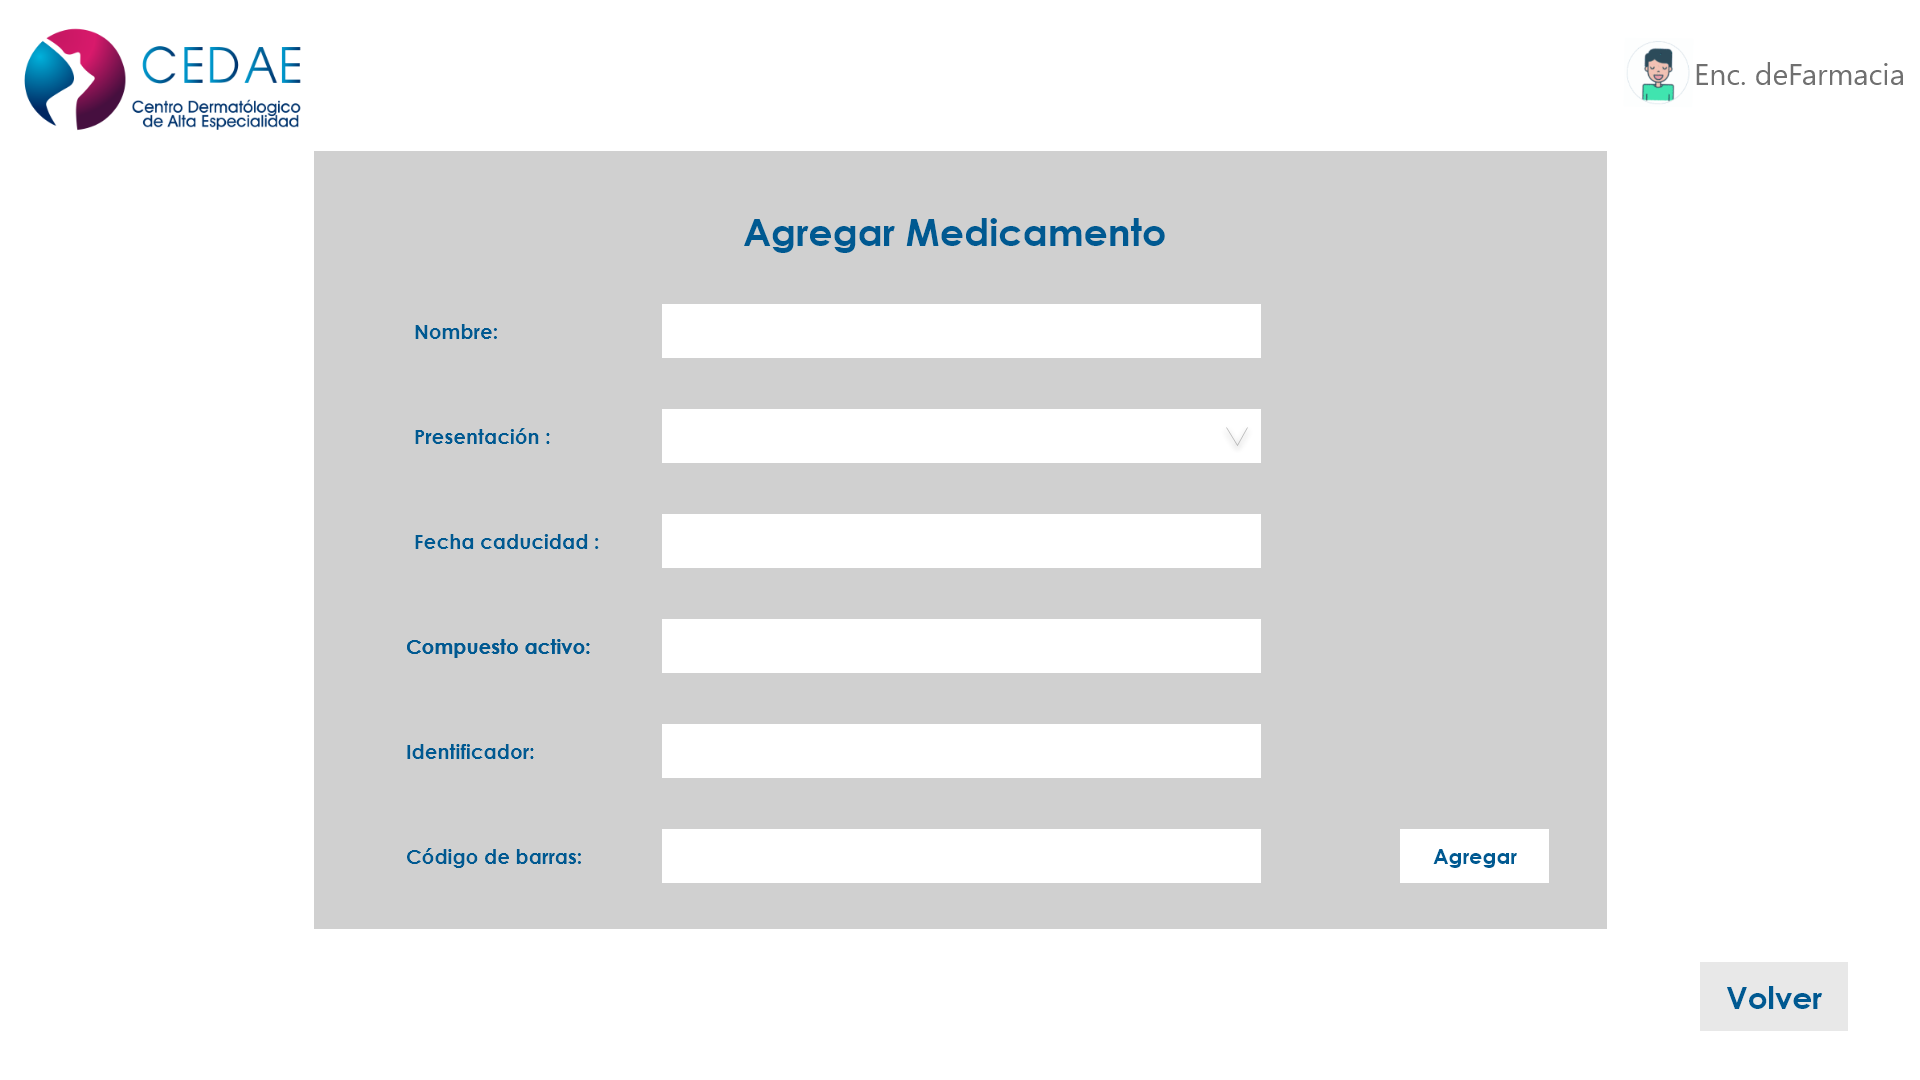
\includegraphics [scale=0.2]{far_add_medicamento}
                \caption{Interfaz de agregar medicamentos}
            \end{figure}
        Eliminar medicamentos
            \begin{figure}[H]
                \centering
                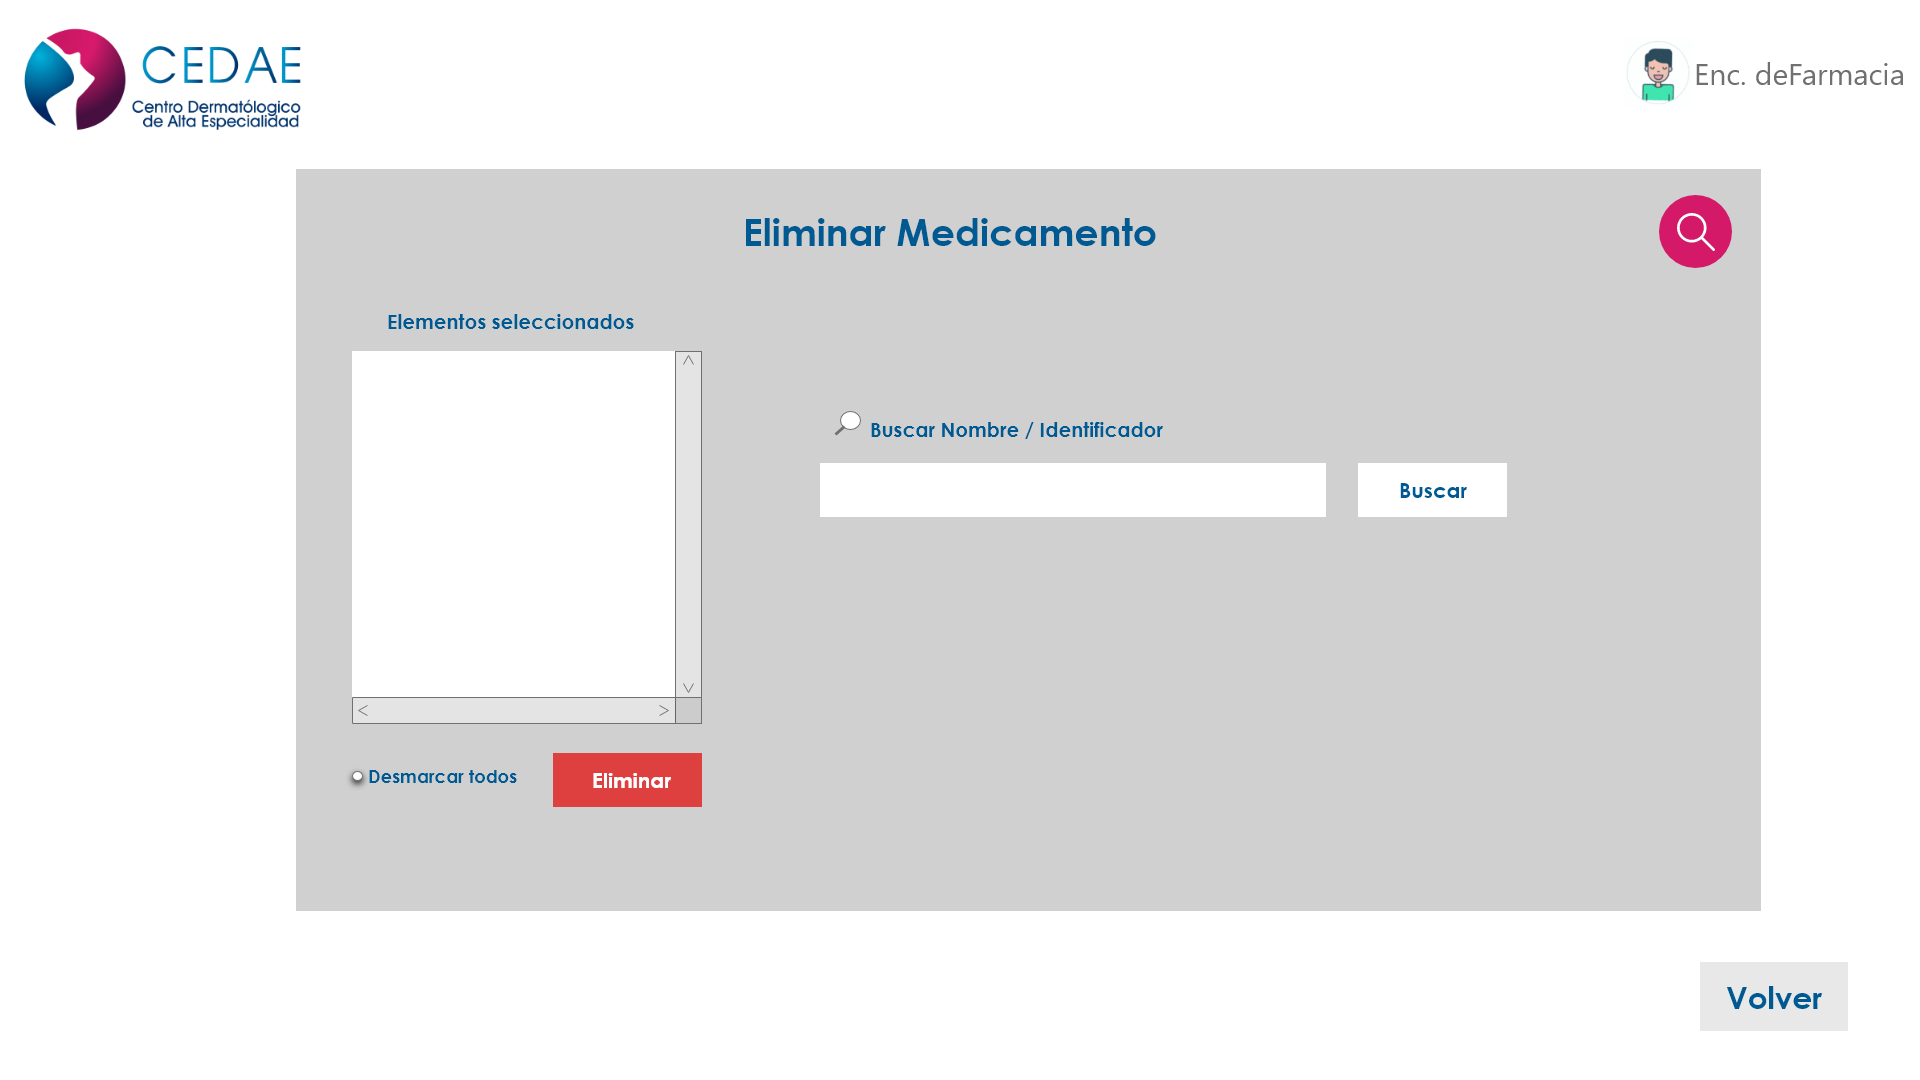
\includegraphics [scale=0.2]{far_delete_medicamento}
                \caption{Interfaz de eliminar medicamentos}
            \end{figure}
        Buscar medicamentos
            \begin{figure}[H]
                \centering
                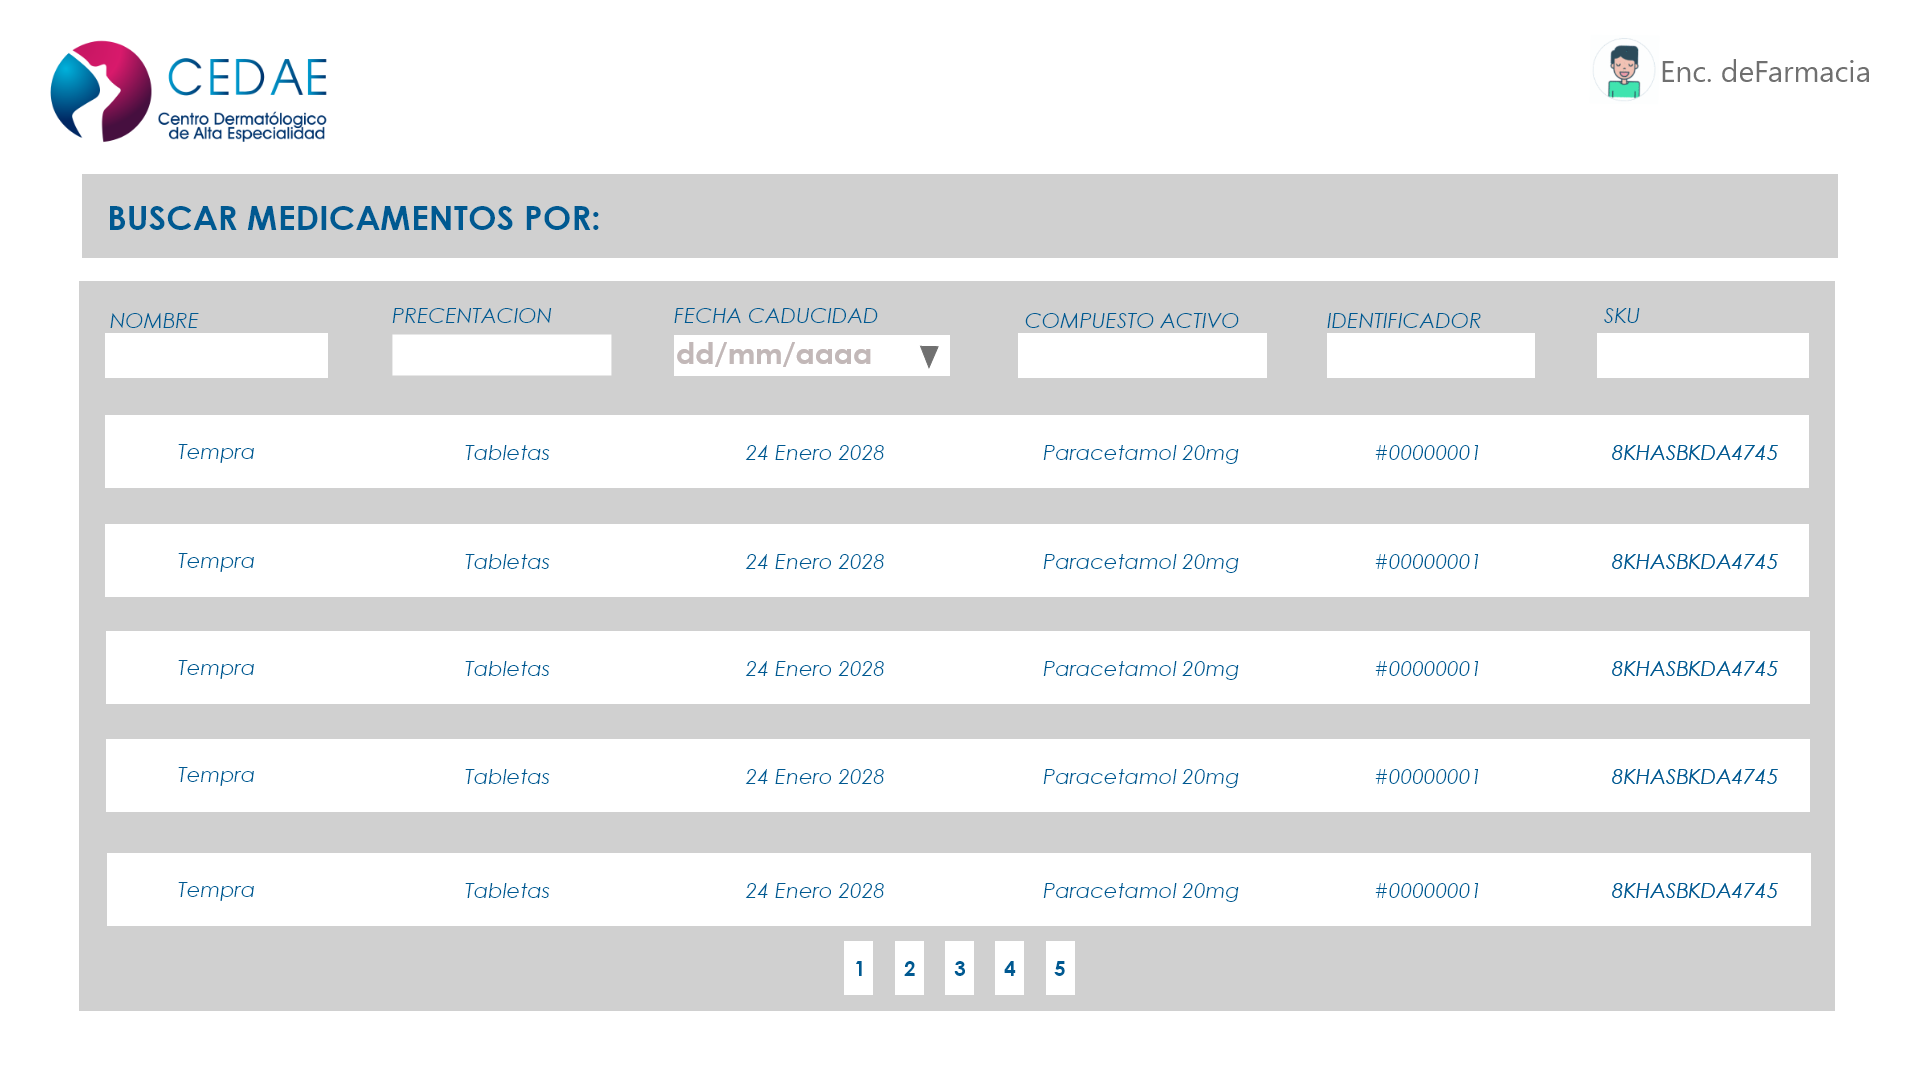
\includegraphics [scale=0.16]{far_bus_medicamento}
                \caption{Interfaz de busqueda de medicamentos}
            \end{figure}
        
        \subsection{Mockups de médico}
        Perfil de médico
            \begin{figure}[H]
                \centering
                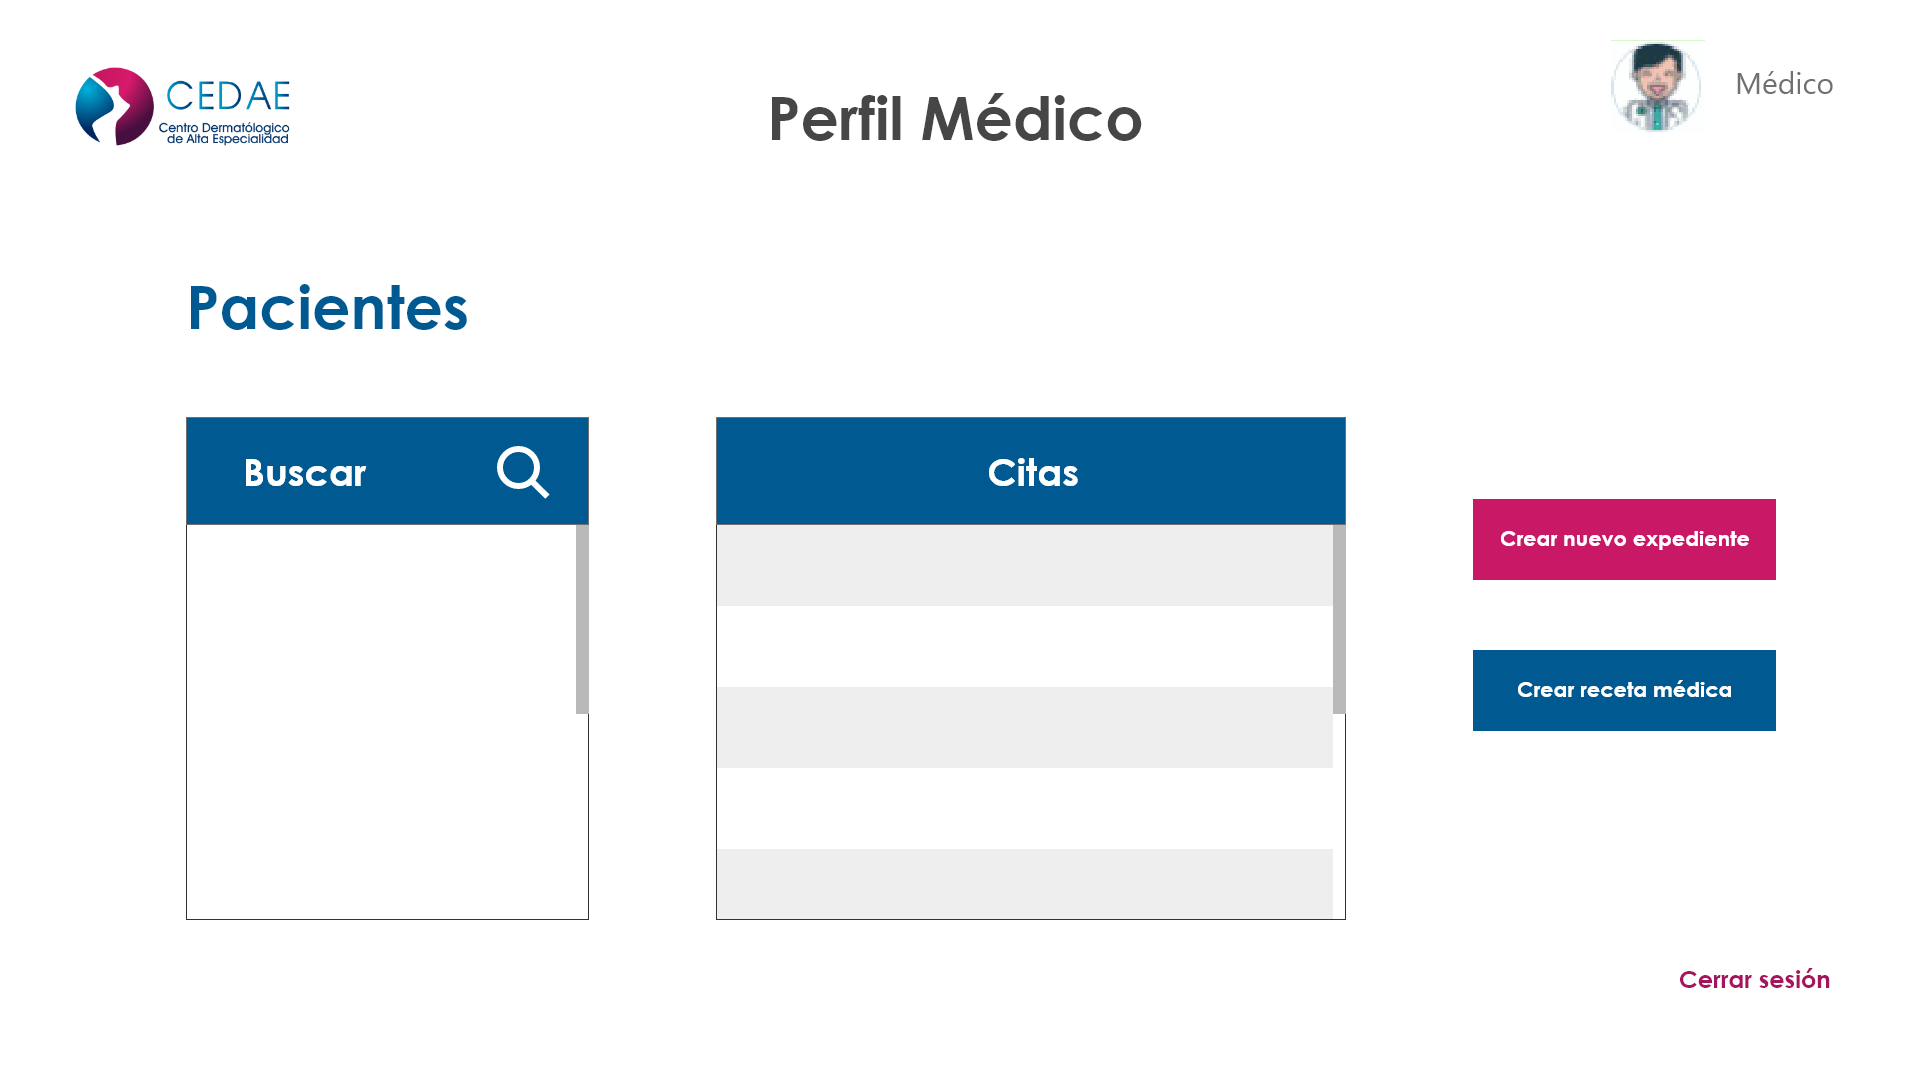
\includegraphics [scale=0.2]{med_perfil}
                \caption{Interfaz de perfil de medico}
            \end{figure}
        Modificar expedientes
            \begin{figure}[H]
                \centering
                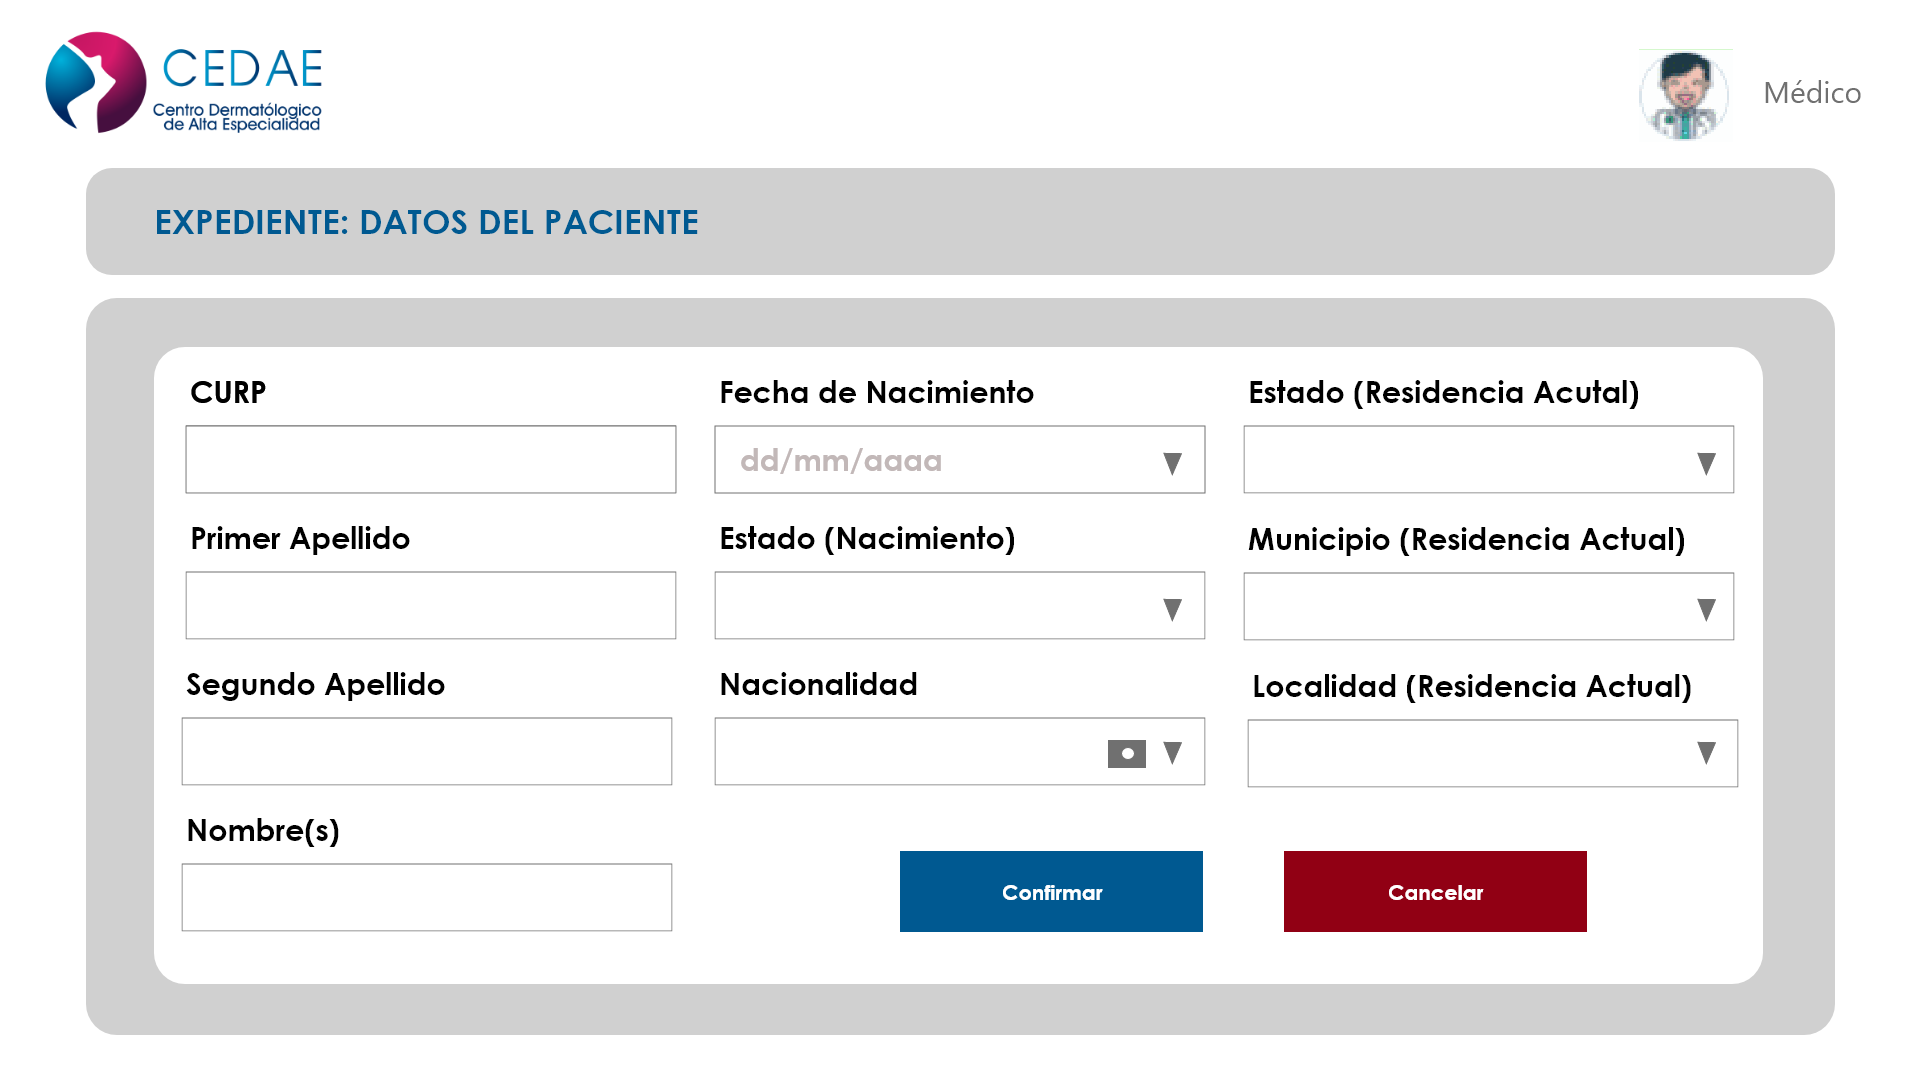
\includegraphics [scale=0.2]{med_mod_expediente}
                \caption{Interfaz de modificación de expedientes}
            \end{figure}
        Ver expedientes
            \begin{figure}[H]
                \centering
                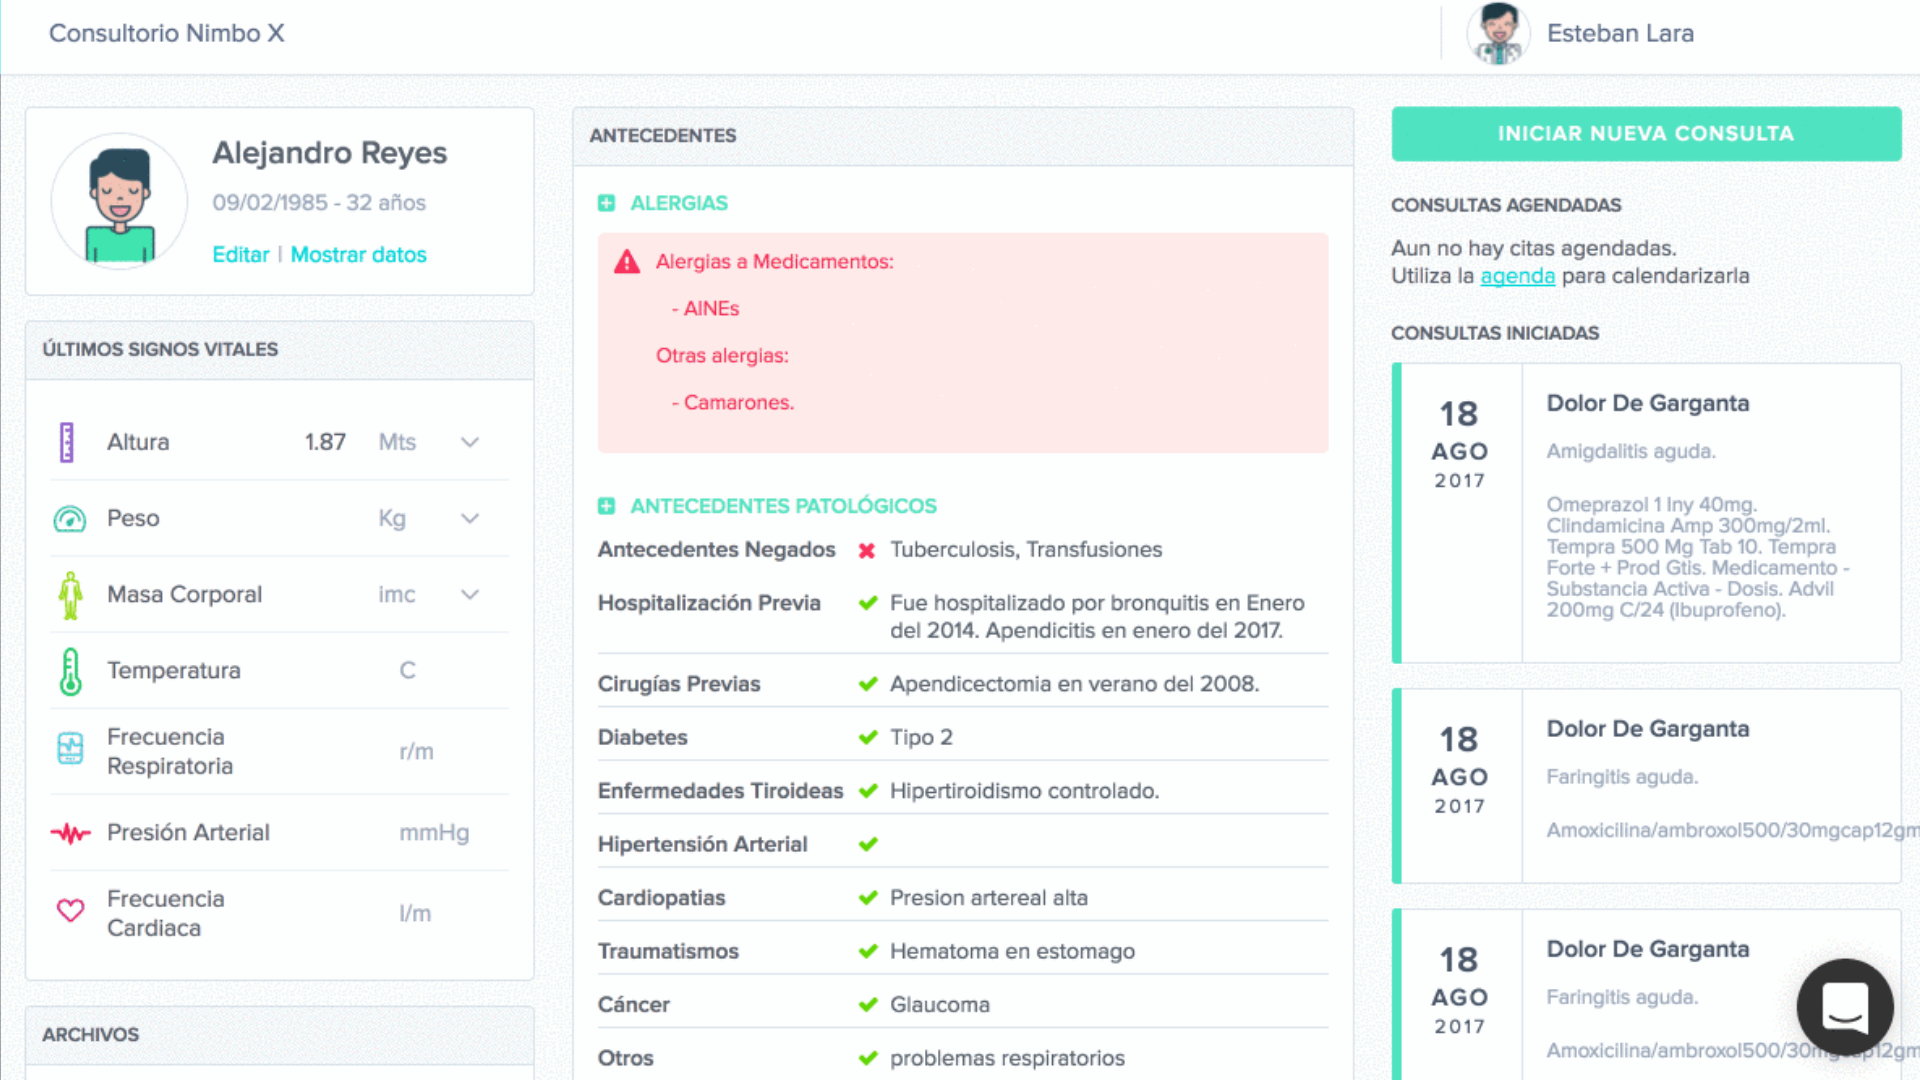
\includegraphics [scale=0.2]{med_ver_expediente}
                \caption{Interfaz de visualización de expedientes}
            \end{figure}
        Citas agendadas
            \begin{figure}[H]
                \centering
                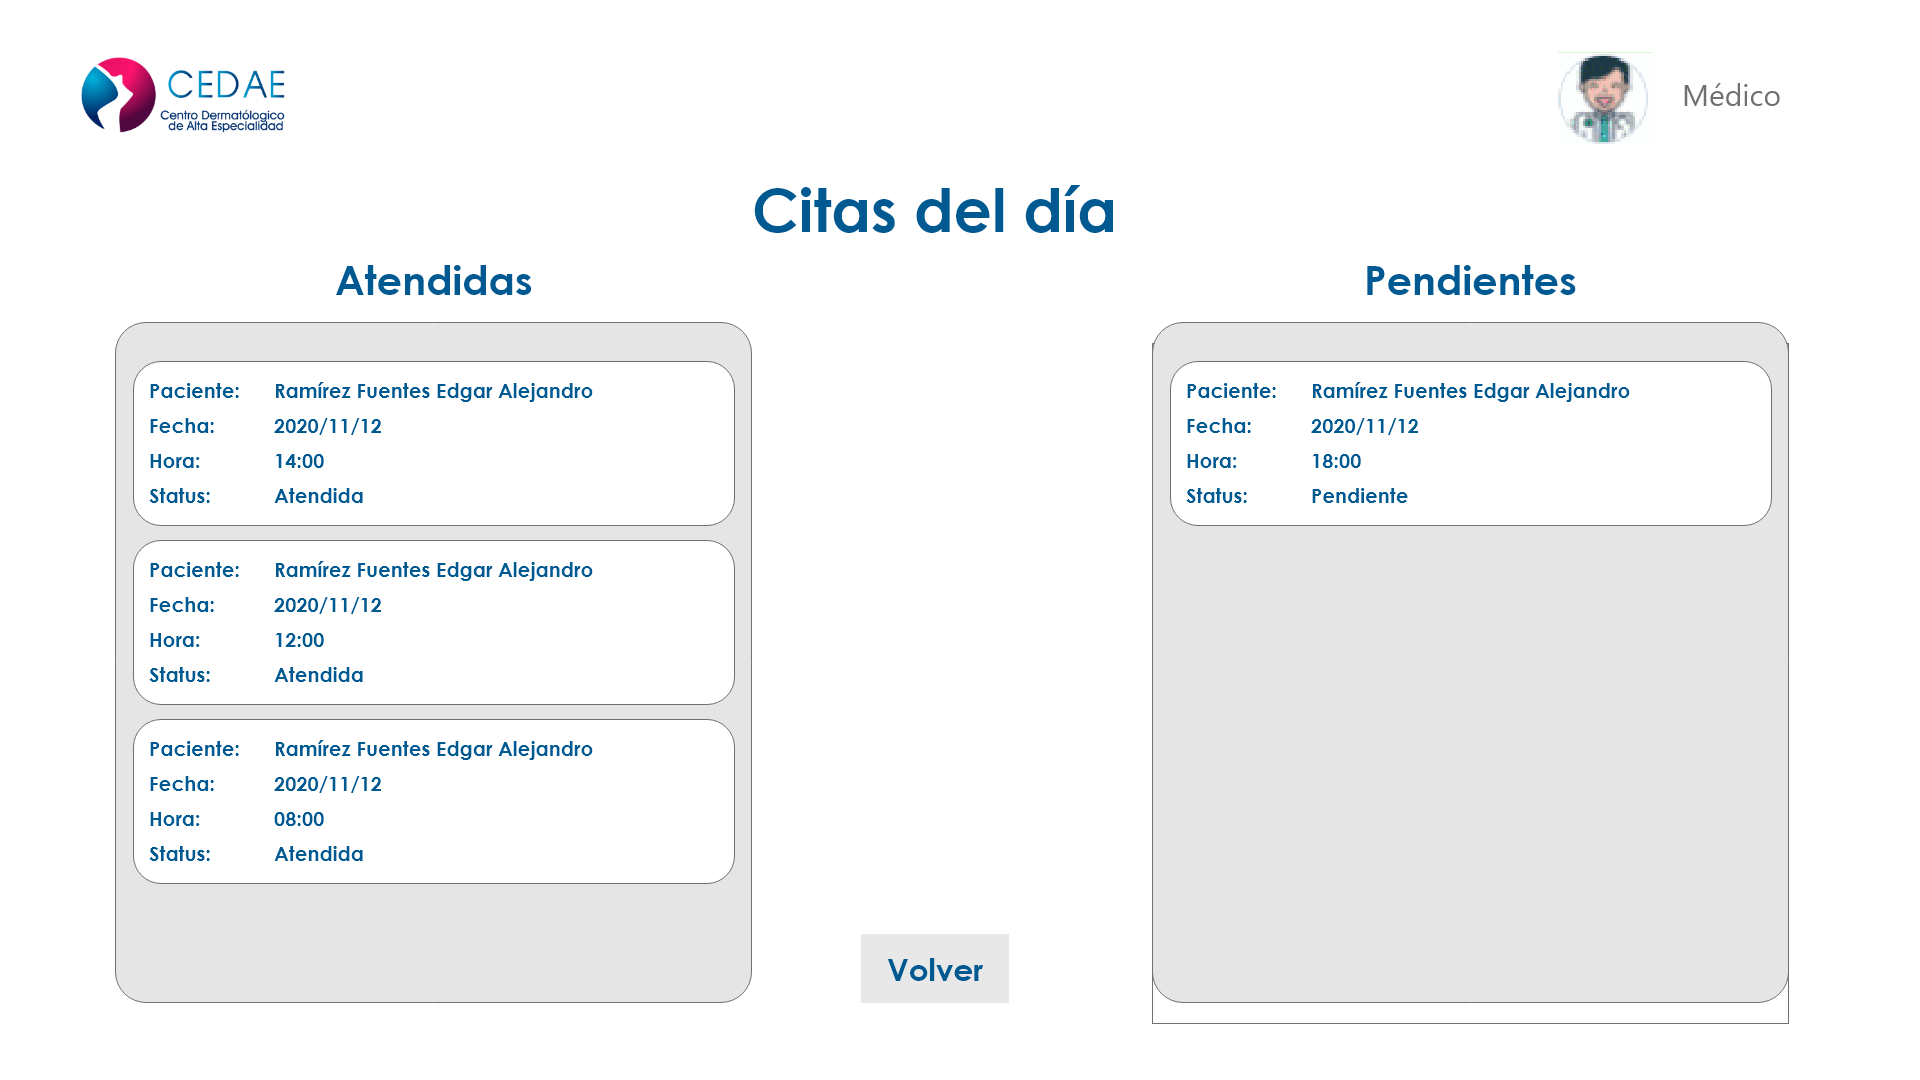
\includegraphics [scale=0.2]{med_ver_citas}
                \caption{Interfaz de citas agendadas}
            \end{figure}
        Crear recetas
            \begin{figure}[H]
                \centering
                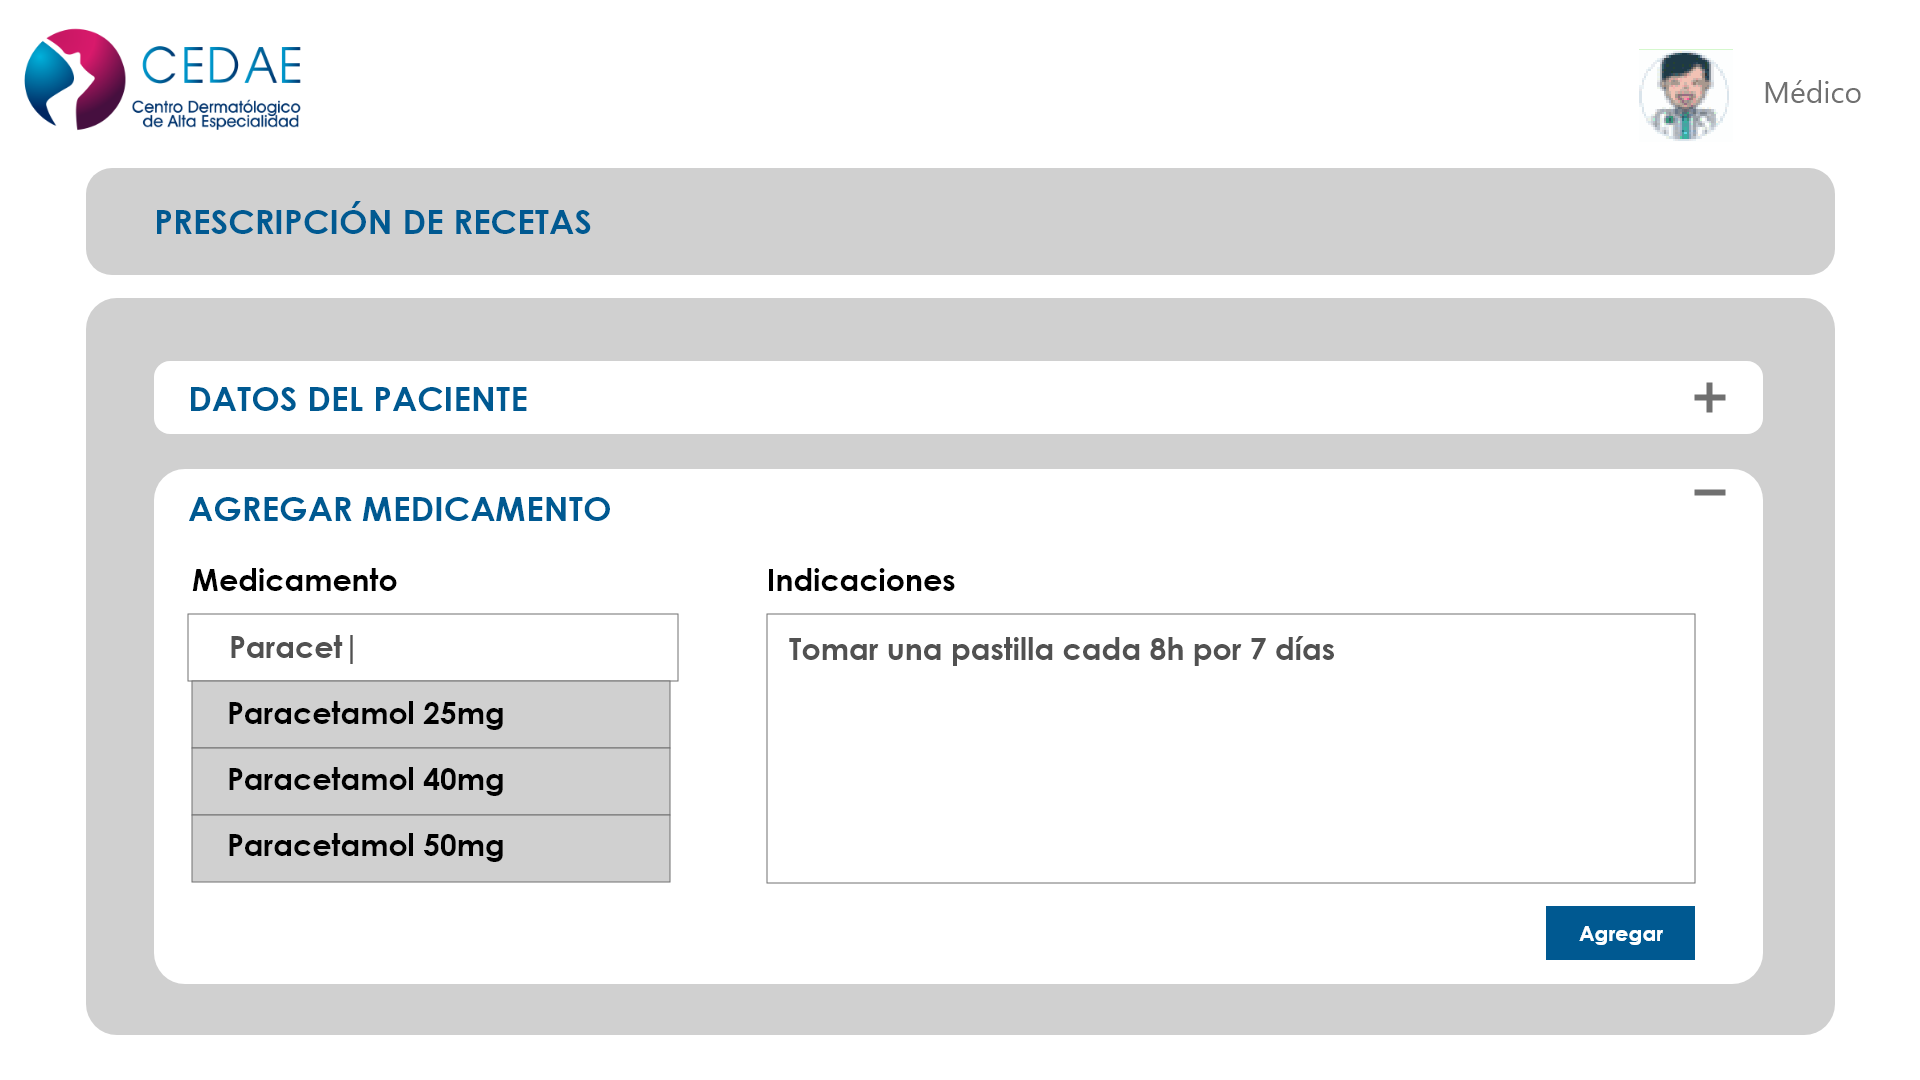
\includegraphics [scale=0.2]{med_crear_receta}
                \caption{Interfaz de creación de recetas}
            \end{figure}

        \subsection{Mockups de paciente}
        Perfil de paciente
            \begin{figure}[H]
                \centering
                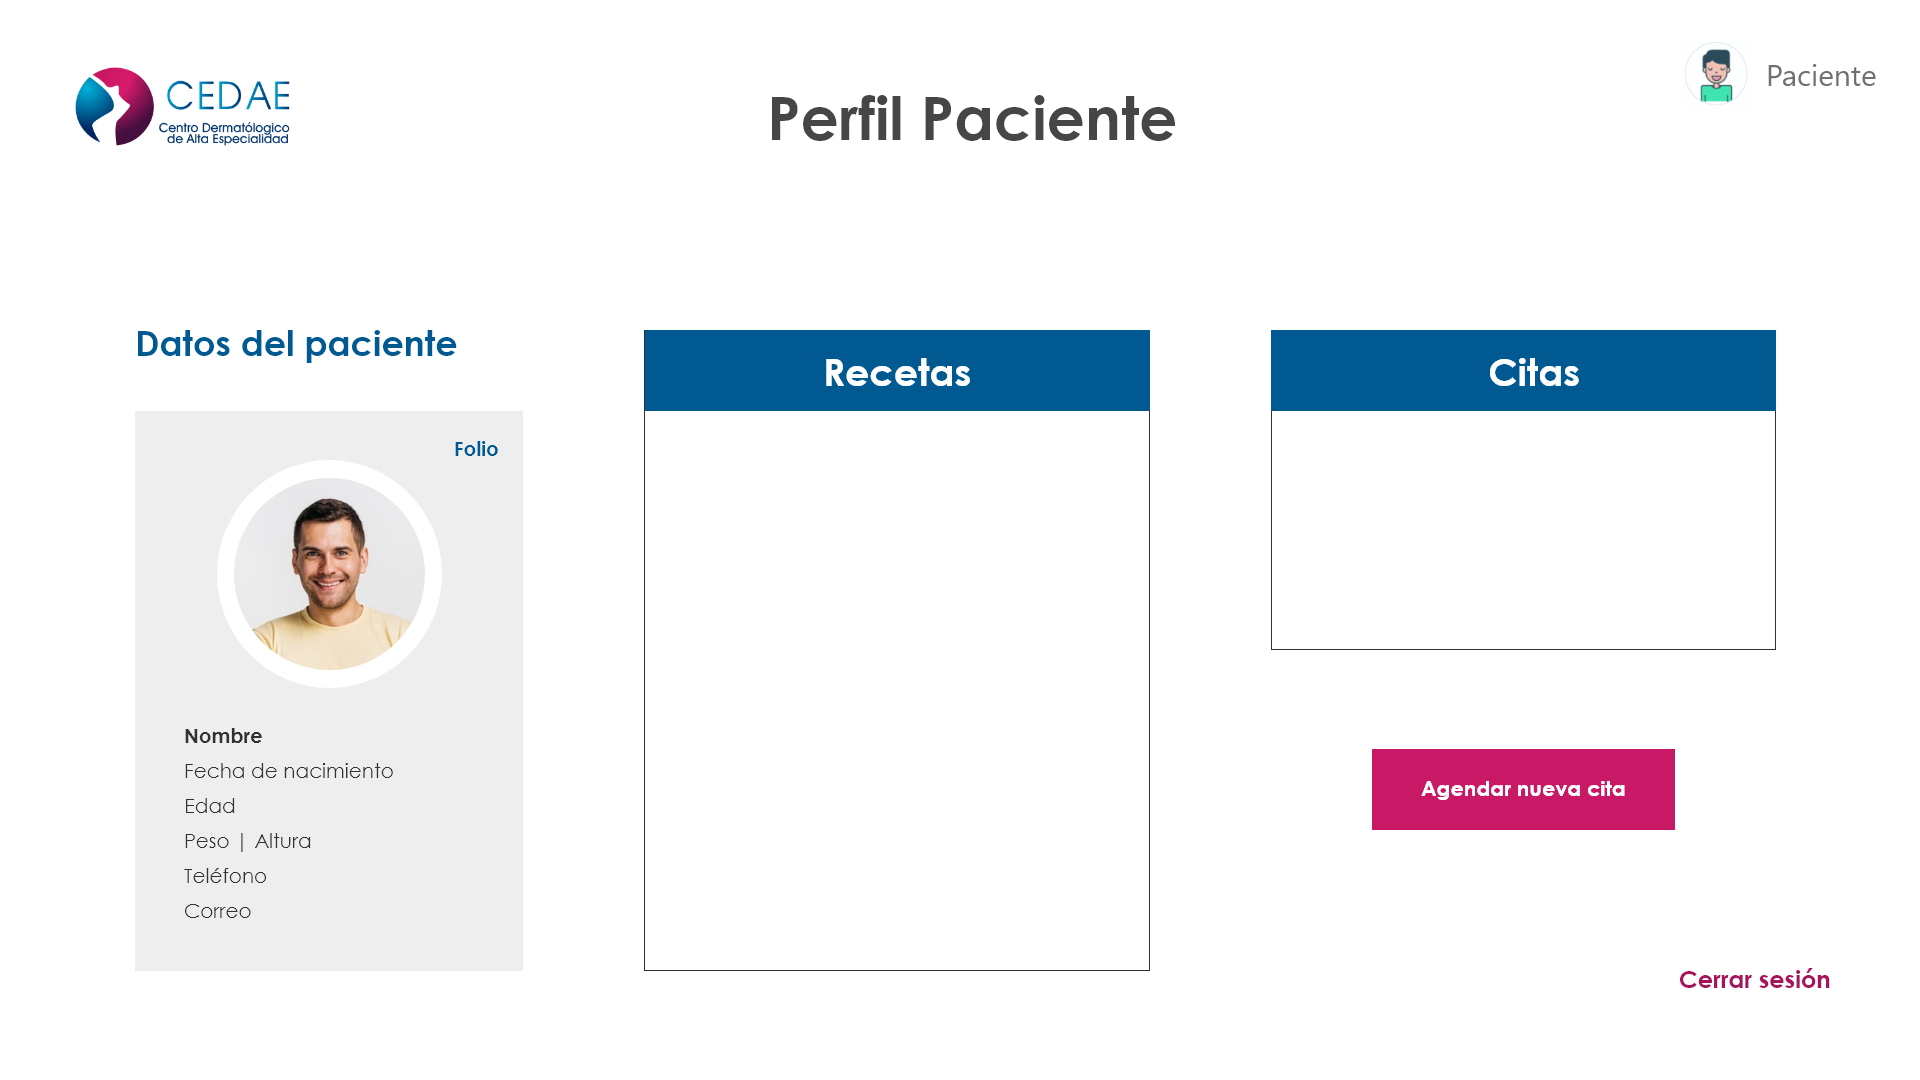
\includegraphics [scale=0.19]{pac_perfil}
                \caption{Interfaz de perfil de paciente}
            \end{figure}
        Agendar cita por primera vez
            \begin{figure}[H]
                \centering
                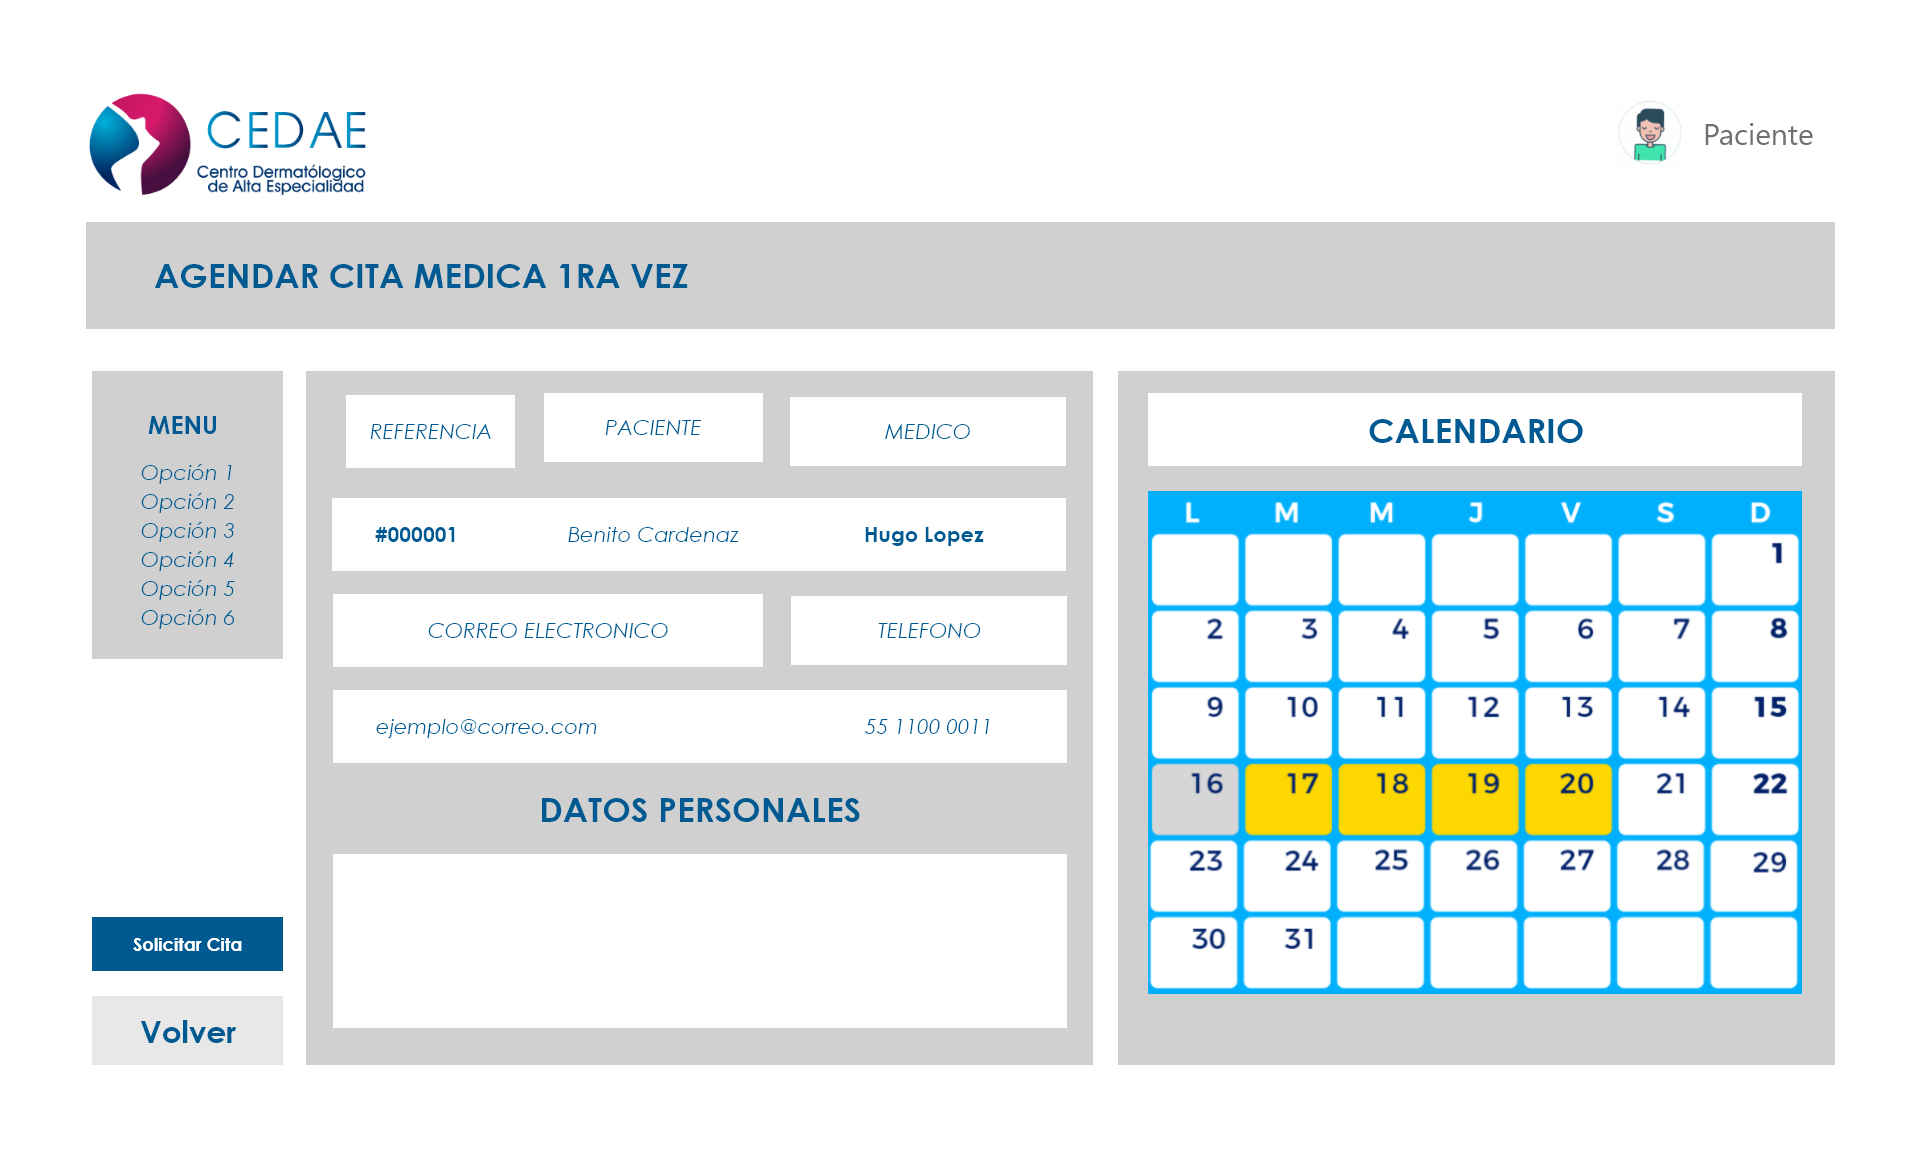
\includegraphics [scale=0.18]{pac_cita_primera}
                \caption{Interfaz de agendar primera cita}
            \end{figure}
        Agendar cita no por primera vez
            \begin{figure}[H]
                \centering
                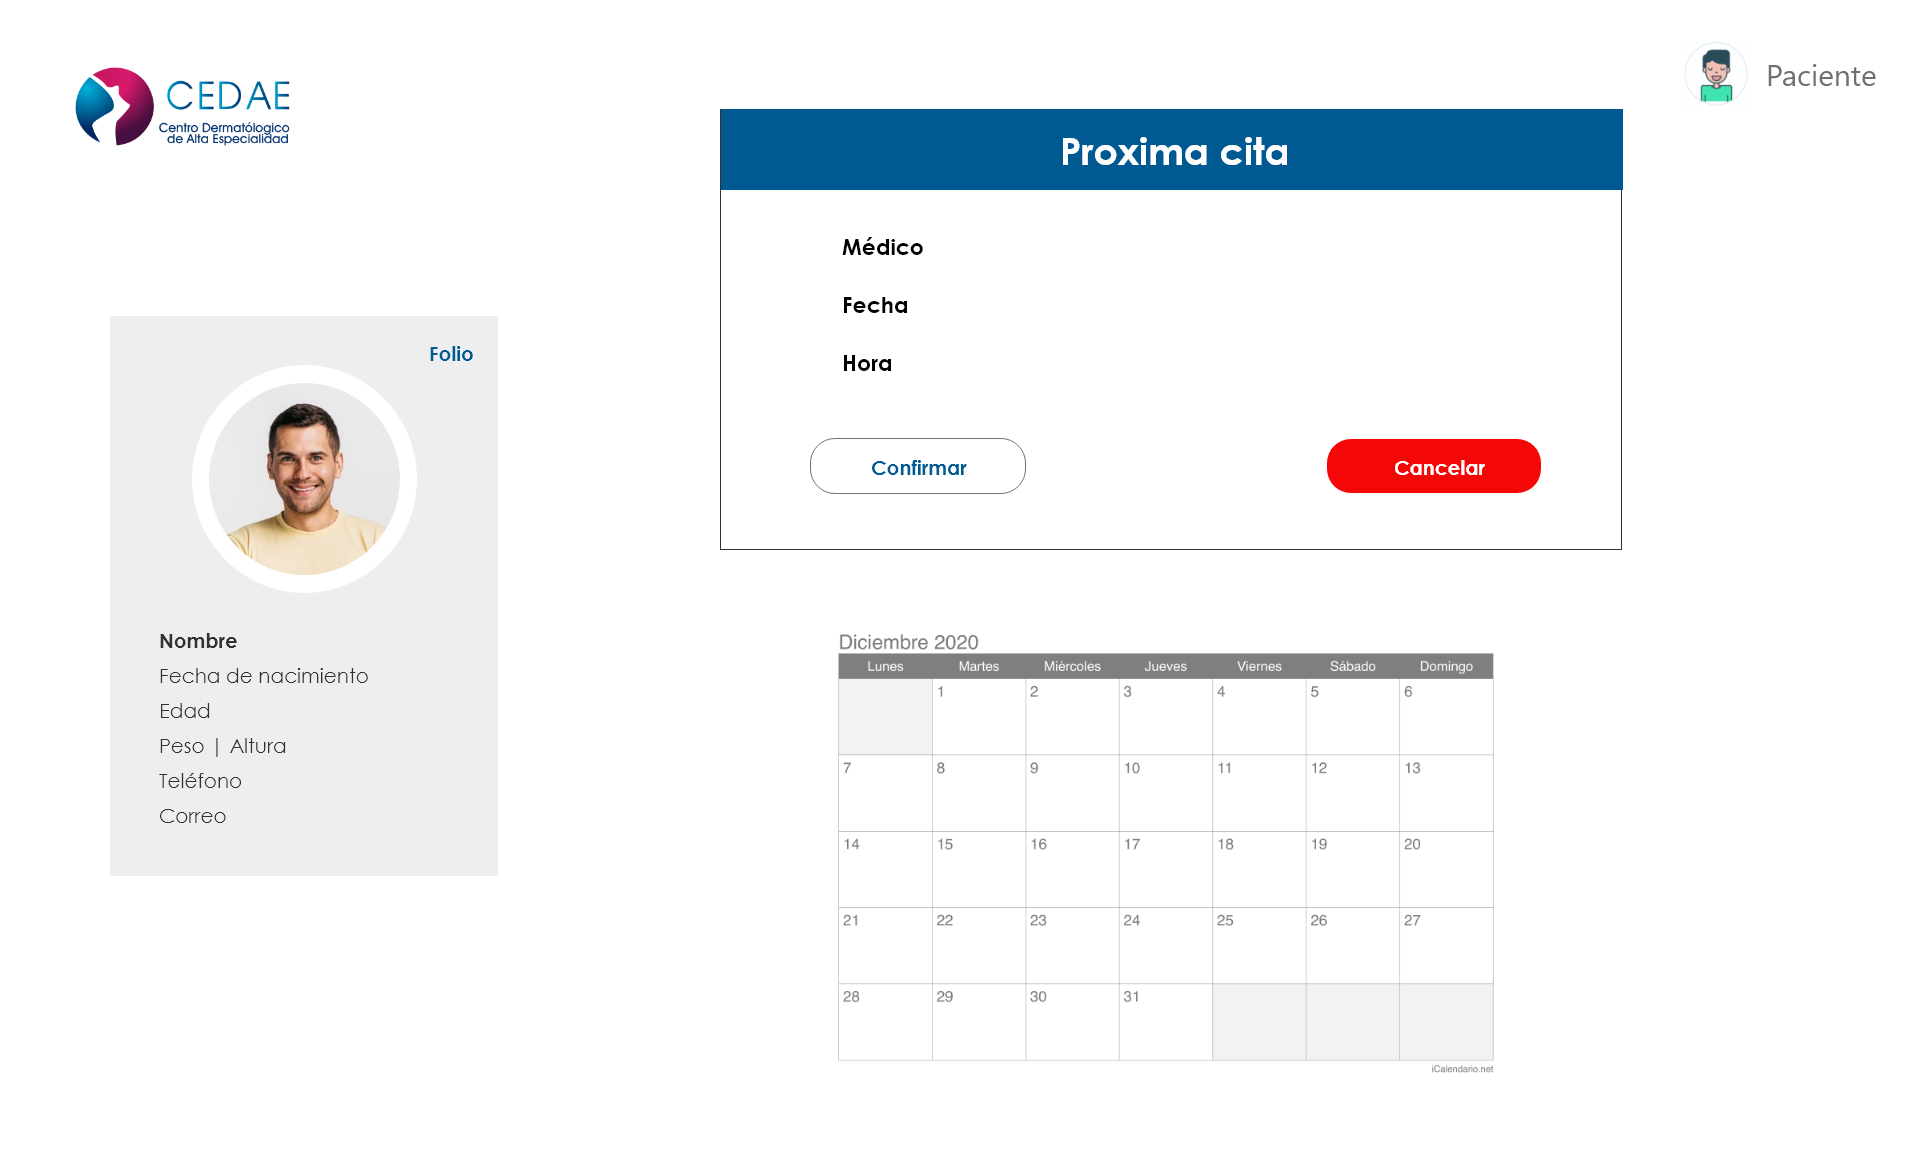
\includegraphics [scale=0.18]{pac_cita_no_primera}
                \caption{Interfaz de agendar cita}
            \end{figure}
        Citas agendadas
            \begin{figure}[H]
                \centering
                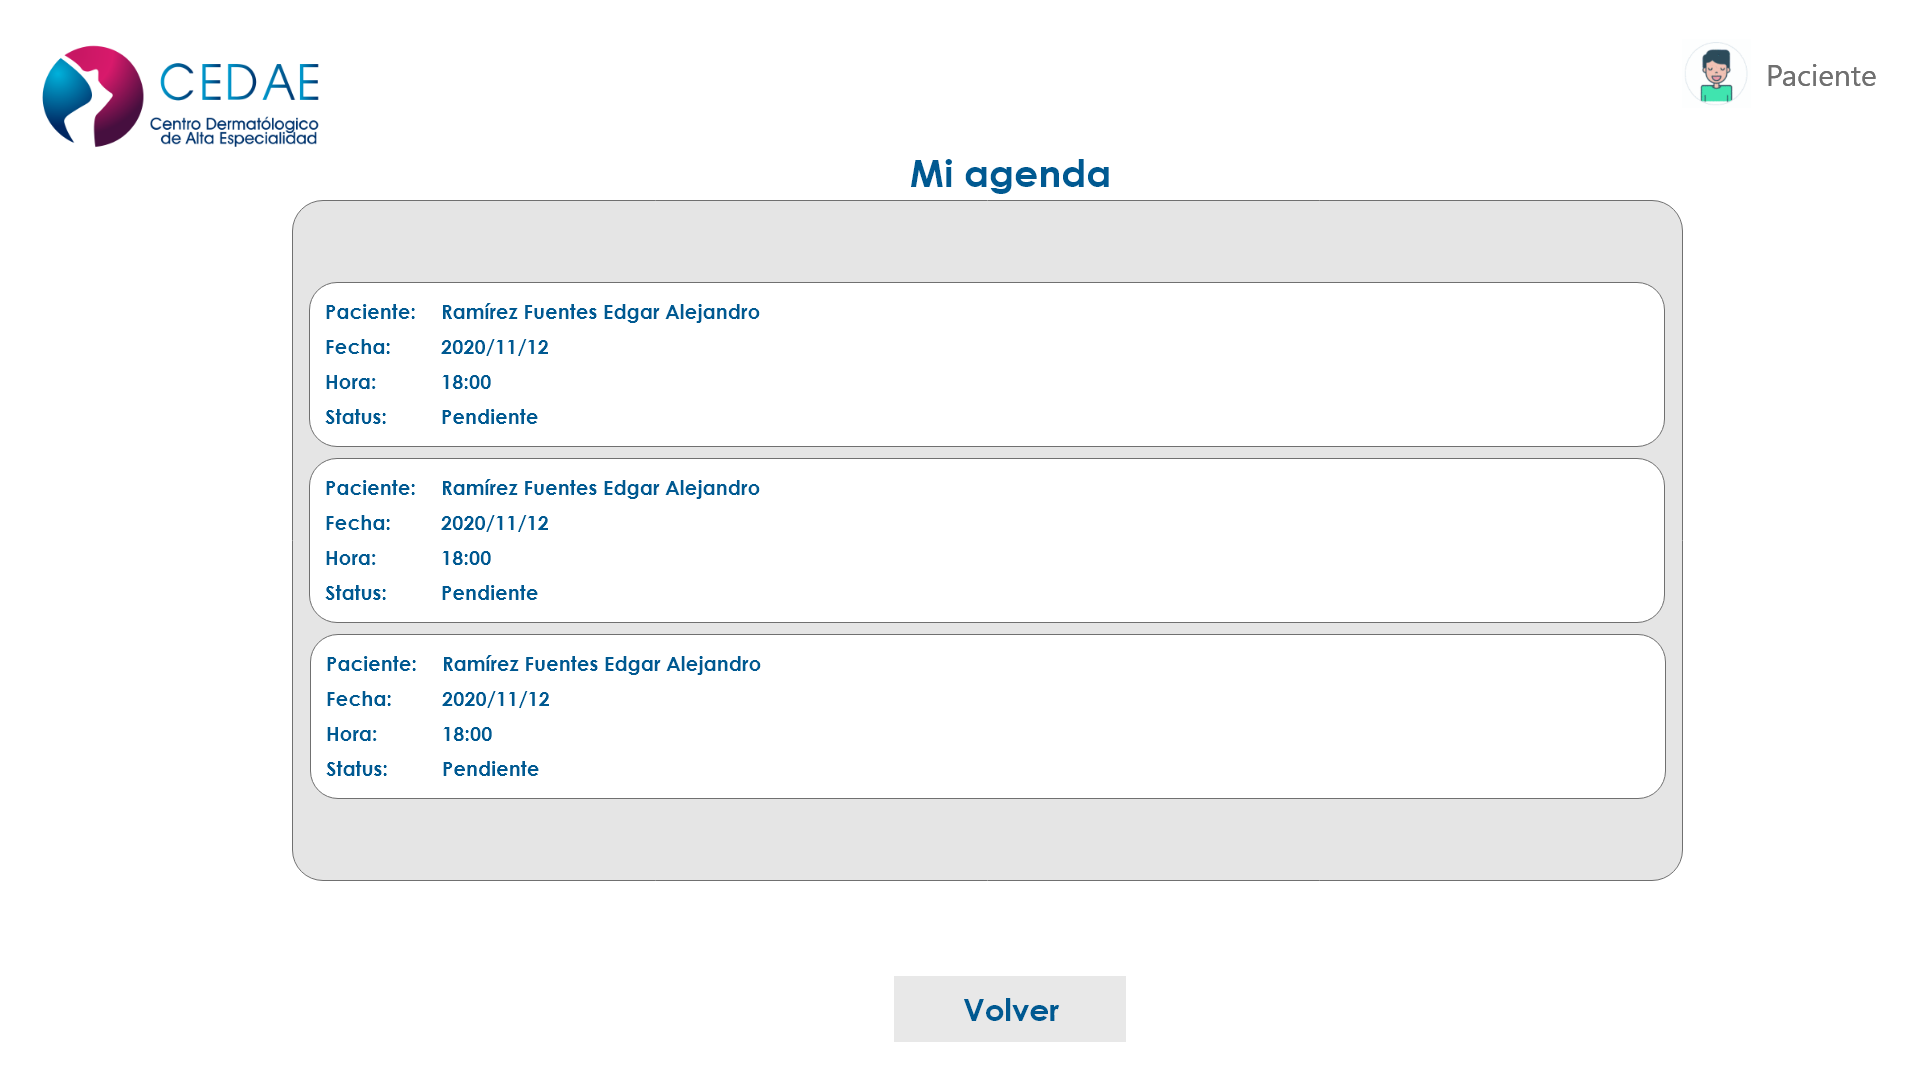
\includegraphics [scale=0.2]{pac_citas_agendadas}
                \caption{Interfaz de citas agendadas}
            \end{figure}

        \subsection{Mockups de recepcionista}
        Perfil de recepcionista
            \begin{figure}[H]
                \centering
                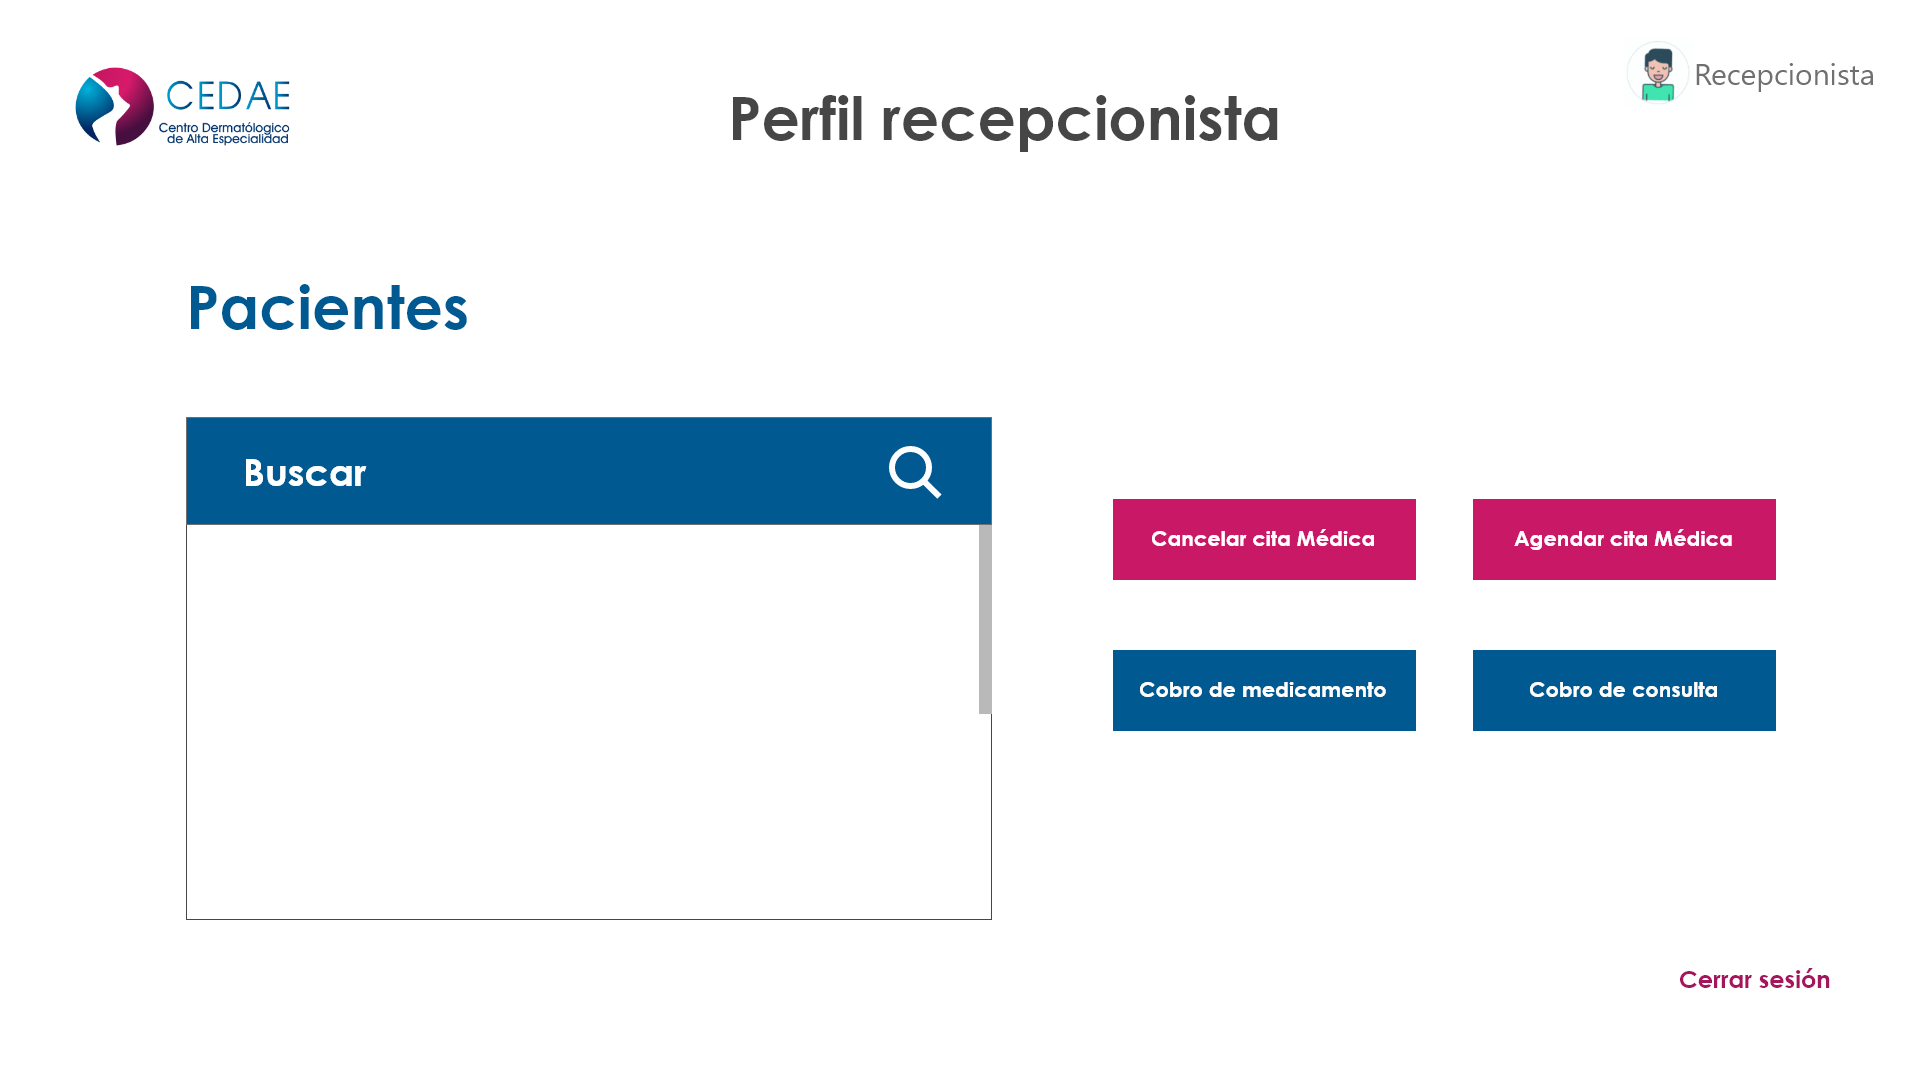
\includegraphics [scale=0.19]{rec_perfil}
                \caption{Interfaz de perfil de recepcionista}
            \end{figure}
        Agendar cita
            \begin{figure}[H]
                \centering
                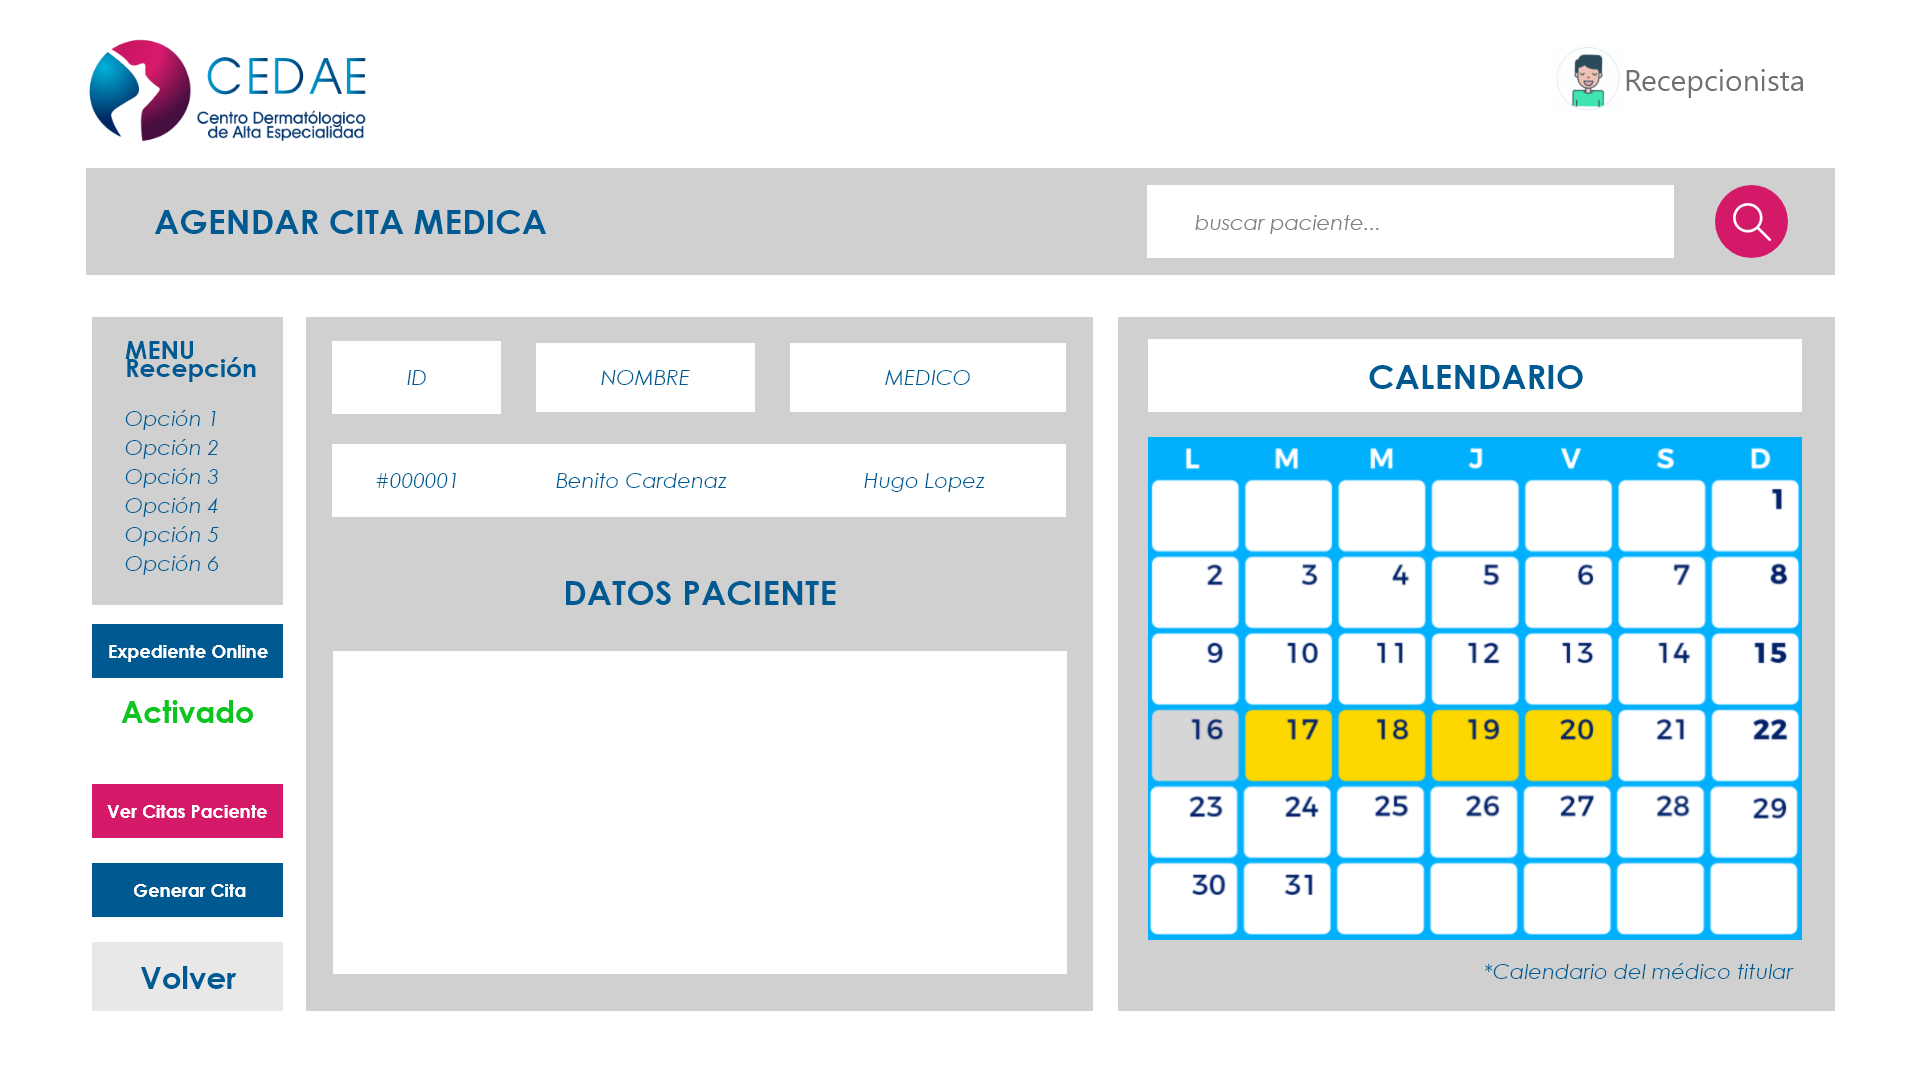
\includegraphics [scale=0.18]{rec_agendar_cita}
                \caption{Interfaz de agendar cita}
            \end{figure}
        Modificar cita
            \begin{figure}[H]
                \centering
                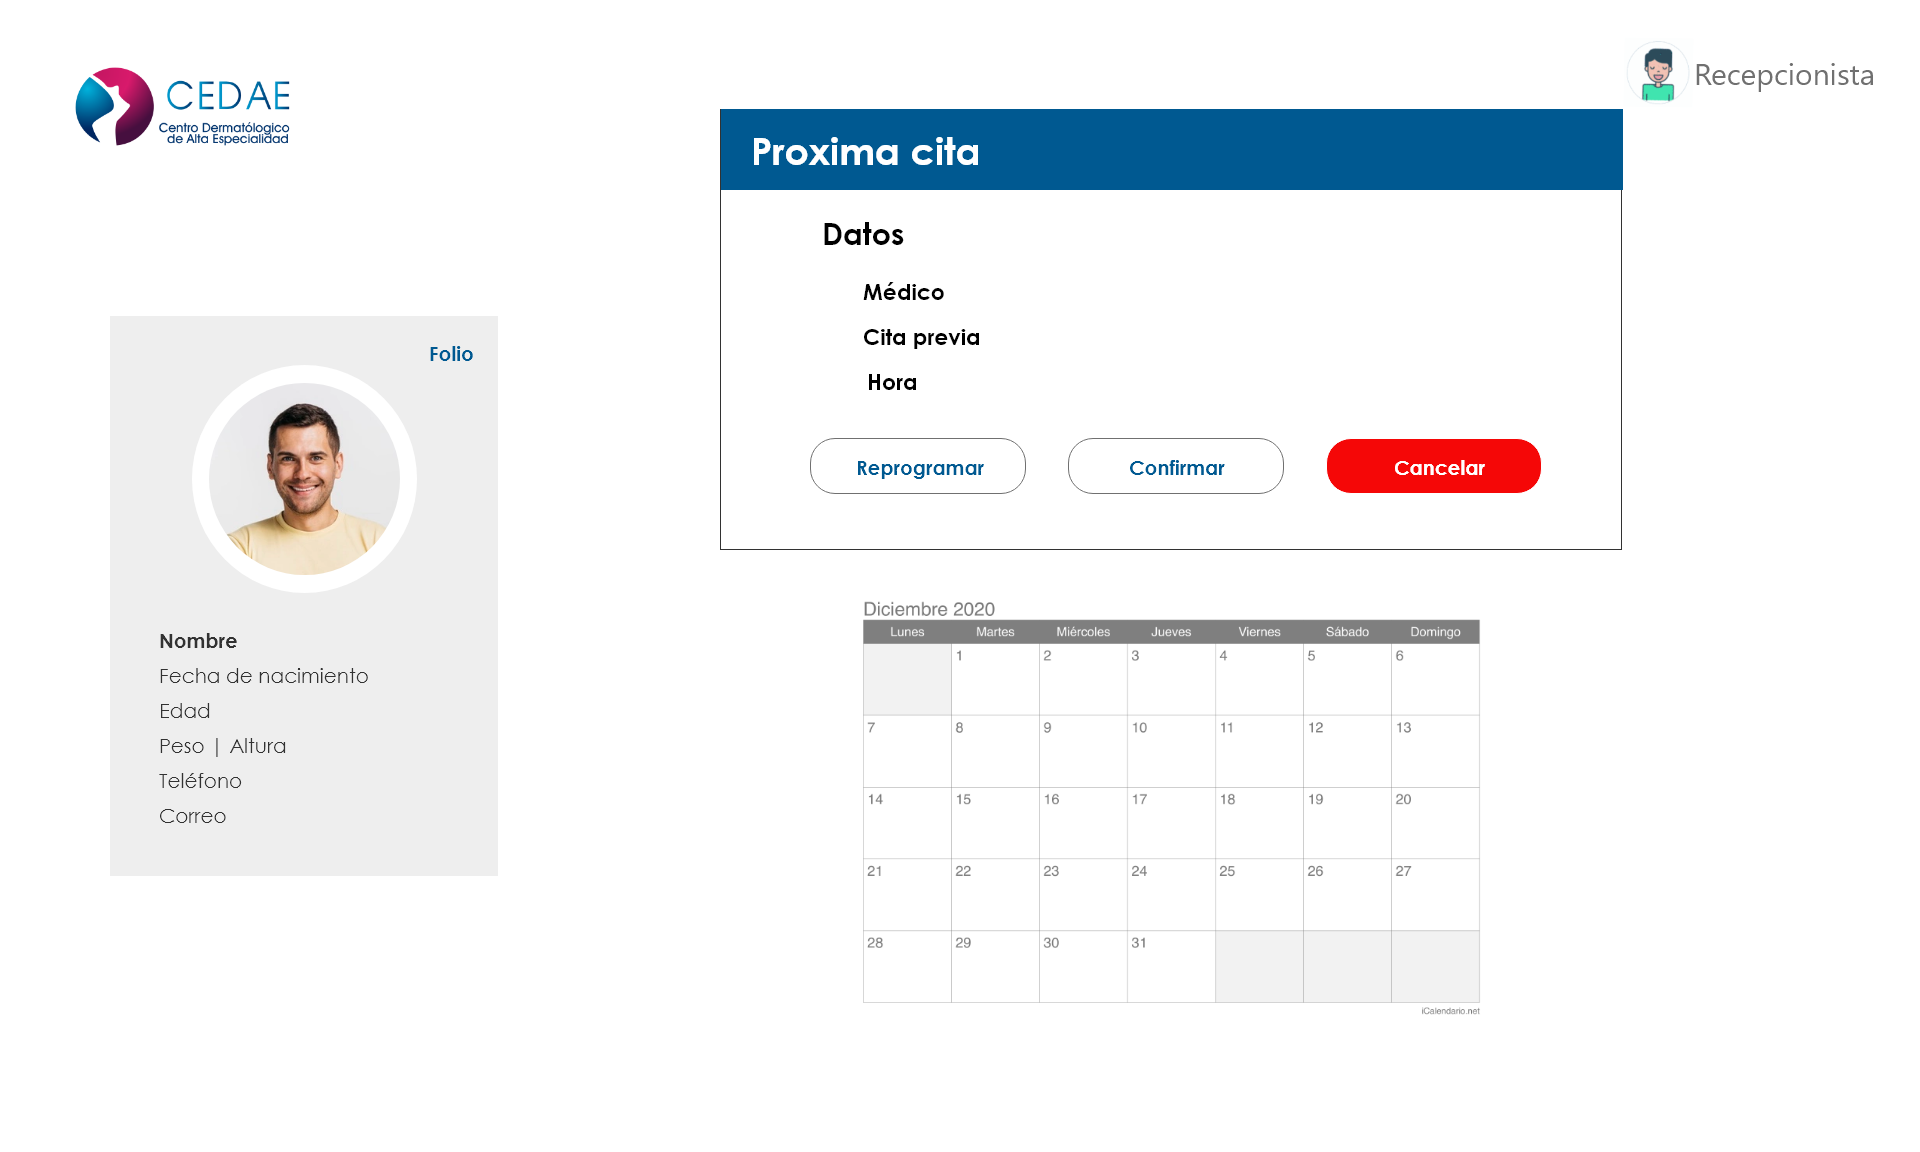
\includegraphics [scale=0.18]{rec_modificar_cita}
                \caption{Interfaz de modificar cita}
            \end{figure}
        Realizar cobros
            \begin{figure}[H]
                \centering
                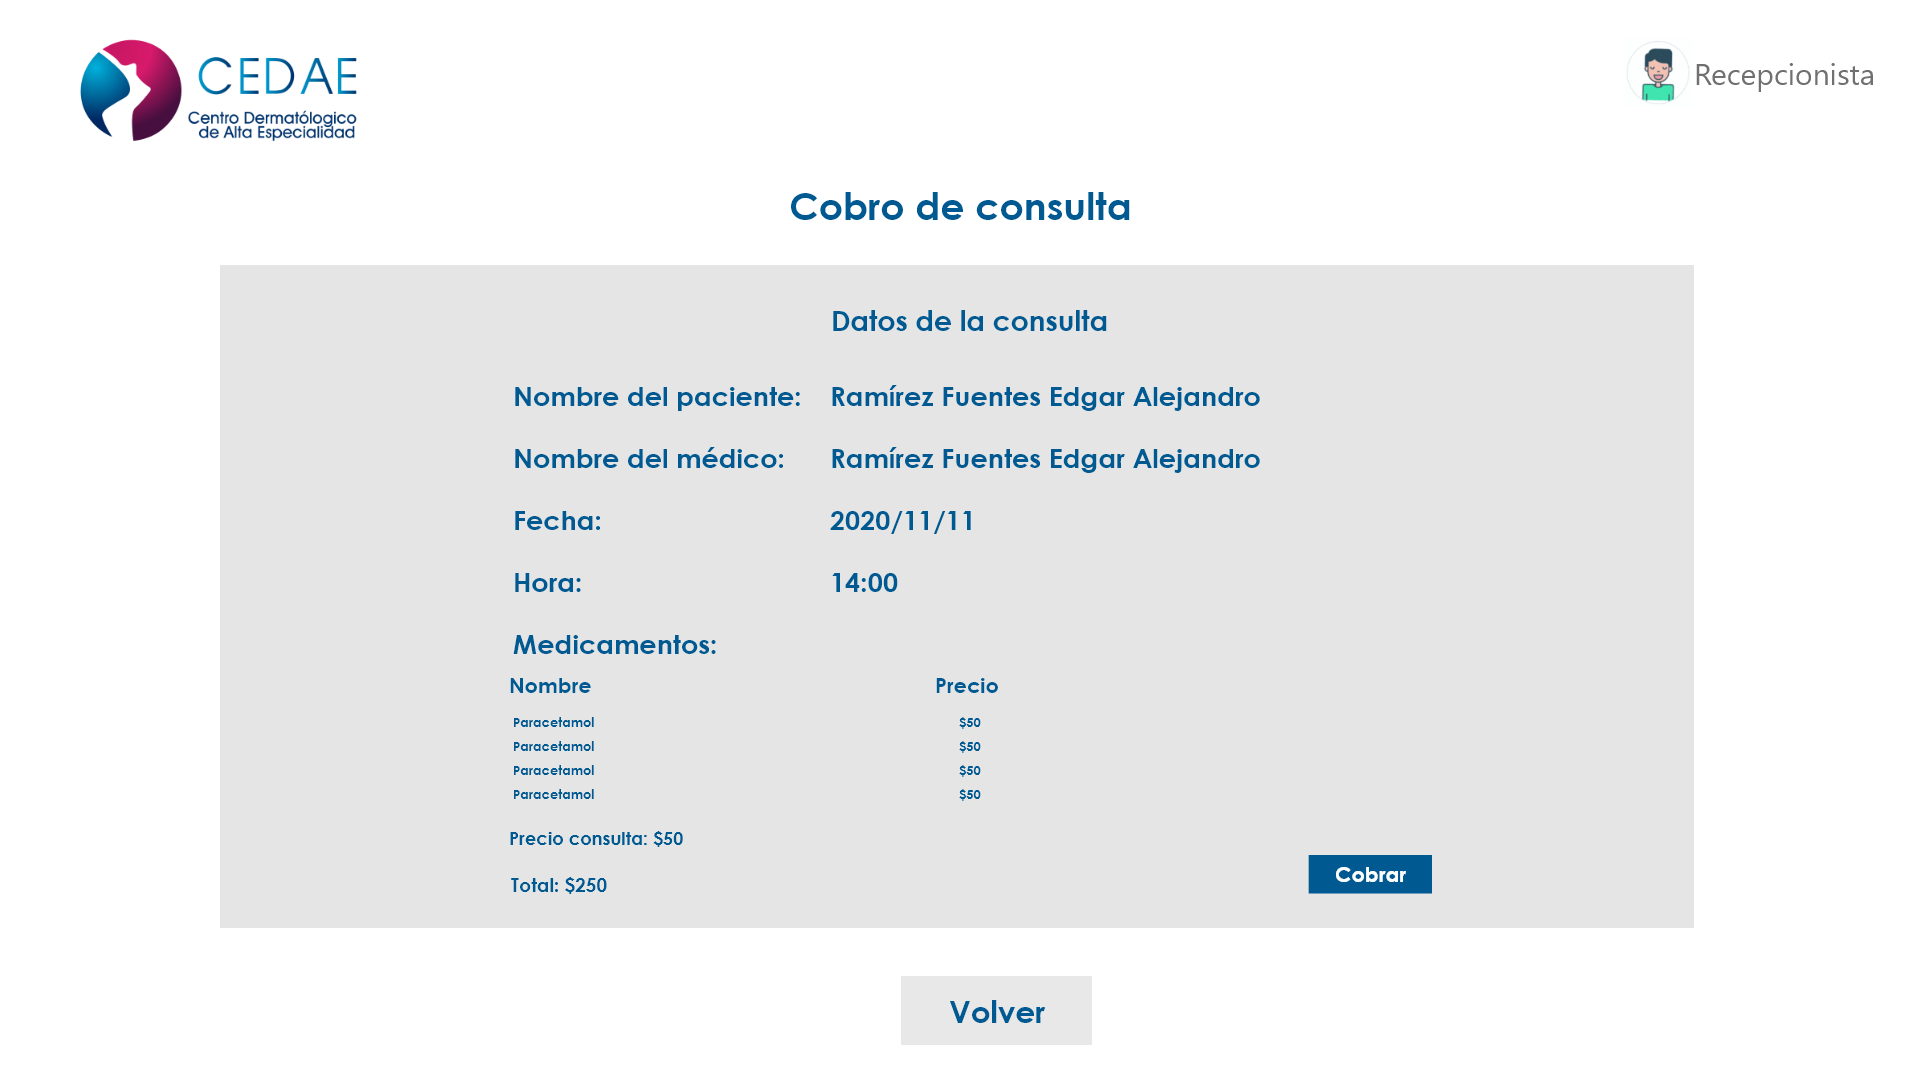
\includegraphics [scale=0.19]{rec_cobro}
                \caption{Interfaz de cobros}
            \end{figure}

\end{document}